\documentclass[conference]{IEEEtran}
%\IEEEoverridecommandlockouts
\usepackage{amsmath,amssymb,amsfonts}
\usepackage{graphicx}
\usepackage{textcomp}
\usepackage{xcolor}
\usepackage{booktabs}
\usepackage{multirow}
\usepackage{array}
\usepackage{url}
\usepackage[breaklinks=true, hidelinks]{hyperref}

\begin{document}

\title{Towards Adversarially Augmented AI Text Detection via Supervised
DistilBERT Fine-Tuning: A Held-Out-Generator Study on RAID}

\author{%
\IEEEauthorblockN{Hammad Masood Mirza}
\IEEEauthorblockA{\textit{Dept. of Artificial Intelligence}\\
\textit{FAST-NUCES, Islamabad}\\
Islamabad, Pakistan\\
madham123098@gmail.com}
\and
\IEEEauthorblockN{Abdul Rafay Rashid}
\IEEEauthorblockA{\textit{Dept. of Artificial Intelligence}\\
\textit{FAST-NUCES, Islamabad}\\
Islamabad, Pakistan\\
rafwas209@gmail.com}}

\maketitle

% ---------------------------------------------------------------
\begin{abstract}
We investigate supervised AI text detection trained on adversarially augmented data and evaluated under a held-out-generator evaluation protocol at consumer-GPU scale. A binary
DistilBERT classifier is fine-tuned on a 120,000-sample balanced subset of
RAID using AI text from seen generators and evaluated on a separate
held-out-generator split containing stronger and commercially deployed model
families. In a single-seed evaluation (seed~42), all four ablation
configurations achieve Relative Robustness Degradation values between
1.1\% and 3.1\%, with held-out F1 ranging from
0.914 to 0.927---within our proposed indicative 5\% generalisation threshold.
Multi-seed replication is needed to confirm these values. The ablation
study shows that the validation-selected configuration
(configuration B) obtains the highest validation and seen-test F1, but
not the strongest robustness profile: the fully unfrozen deep-head variant
(configuration C) achieves the best held-out ROC-AUC and nearly tied
held-out F1, while the single-head models achieve the lowest degradation.
Four systems optimisations
are implemented and benchmarked on a single RTX~4050 6~GB GPU: parallel
preprocessing ($3.58\times$ speedup), optimised DataLoader pipeline, AMP training
with enlarged batch size ($3.32\times$ speedup), and AMP inference mode (54.25\%
latency reduction, 380.64 samples/second). As auxiliary contributions,
GPT-2 XL Perplexity is reproduced with AUROC 0.937 and extended with 4-bit NF4
quantisation on RAID adversarial subsets, demonstrating that
clean-benchmark performance degrades sharply under adversarial attack
(AUROC 0.526--0.789), with homoglyph substitution more destructive than paraphrase rewriting:
the additional AUROC degradation from paraphrase to homoglyph reaches 33.40\% for GPT-2 XL
and 14.99\% for GPT-J-6B, respectively.
\end{abstract}

\begin{IEEEkeywords}
adversarial robustness, AI text detection, DistilBERT, held-out-generator
generalisation, RAID, NF4 quantisation, efficient inference
\end{IEEEkeywords}

% ---------------------------------------------------------------
\section{Introduction}\label{sec:intro}

Large language models (LLMs) such as GPT-4 and LLaMA make fluent, human-sounding
text straightforwardly producible at scale. This capability threatens domains dependent
on content authenticity, particularly academia and journalism, where machine-generated
submissions bypass standard verification. Human inspection fails; research shows
people detect AI-generated text at rates barely above chance~\cite{ippolito2020}.
Automated detection is therefore a critical scalable response.

Two dominant paradigms have emerged for automated detection.
\textbf{Zero-shot probability-based methods} such as GPT-2 XL Perplexity~\cite{bao2024}
and Binoculars~\cite{hans2024} require no labelled training data. They measure
whether a text occupies a high-probability region of an LLM's output distribution,
achieving AUROC values exceeding 0.98 on clean benchmarks. However, the RAID
benchmark~\cite{dugan2024} (an adversarial evaluation spanning 6.2~million samples,
11~LLMs, and 11~attacks) showed this class of detector is fragile. Homoglyph
substitution alone caused accuracy drops of up to 40.6\% for specific detectors.
The vulnerability is architectural. Any surface-level manipulation that shifts
token log-probabilities directly disrupts the probability-based detection signal.

\textbf{Supervised fine-tuning} addresses this fragility by hypothesis: a
model trained on labelled human and AI text learns stylistic representations
distributed across encoder weights instead of relying on surface probability
statistics. Such representations are harder to fool through adversarial
token-level perturbation. However, Huang et al.~\cite{huang2024} challenged
this assumption. They found that training on adversarially augmented data does
not automatically generalise robustness to unseen attack types, and may actively
worsen cross-attack robustness relative to a clean-trained baseline. This
\emph{cross-attack generalisation gap}---whether supervised adversarial training
on one class of attacks produces models robust to a mechanistically distinct
class---remains open in the literature.

We investigate whether a DistilBERT-based~\cite{sanh2019} binary text
classifier, fine-tuned on a stratified subset of RAID, retains robustness
when evaluated on AI text from generators withheld from training. The
experimental design is conservative at the model-family level: training uses
open-source or older seen generators, while held-out evaluation uses stronger
and commercially deployed generators. Because RAID also contains multiple
adversarial transformations, this protocol tests whether supervised
fine-tuning on adversarially augmented RAID data transfers to a distinct
generator family rather than merely memorising a narrow source distribution.

We select DistilBERT at 66~million parameters for two reasons. Practically,
it is a compact model deployable within the 6~GB VRAM constraint of
the experimental hardware. Scientifically, verifying whether held-out-generator
robustness persists at compressed parameter scale is an independent
contribution. Larger adversarially robust models in the literature (e.g.,
GREATER by Li et al.~\cite{li2025}) require hardware inaccessible in
consumer-grade settings.

The systems contribution of this paper addresses the engineering required to
train four ablation configurations on 120,000~samples over three epochs on a
single consumer GPU. We implement and evaluate four systems optimisations:
parallel multi-stage dataset preprocessing (PP),
an optimised DataLoader pipeline (DLO), Automatic Mixed Precision training (AMP-T),
and AMP-combined inference-mode acceleration (AMP-I). We benchmark these
optimisations against sequential baselines to quantify efficiency gains.

This paper also integrates two auxiliary empirical contributions against a
GPT-2 XL Perplexity baseline. First, we reproduced the original paper's
ChatGPT/GPT-4 aggregate AUROC (0.937 vs.\ the paper's 0.9338 target) to
confirm implementation fidelity. Second, we extended GPT-2 XL Perplexity with
4-bit NF4 quantisation and evaluated it on RAID homoglyph and paraphrase
subsets. This provides an adversarial characterisation of this
detector under the RAID benchmark's attack conditions.

\smallskip
\noindent\textbf{Research Questions.} This paper addresses two primary
questions:

\smallskip
\noindent\textbf{RQ1:} Does a DistilBERT model trained on adversarially augmented RAID data
text from seen generators retain robustness on held-out generators, and how
does its held-out performance compare with zero-shot probabilistic detectors
under RAID adversarial conditions? (The comparison is inherently directional
because the supervised and zero-shot paradigms use different primary metrics
---held-out F1 vs.\ adversarial AUROC---and are evaluated on distinct RAID splits.)

\smallskip
\noindent\textbf{RQ2:} How do classification head depth and encoder
fine-tuning depth independently affect seen-generator detection accuracy and
held-out-generator robustness?

\smallskip
The remainder of this paper is organised as follows. Section~\ref{sec:bg}
reviews relevant background and prior systems. Section~\ref{sec:model}
describes the model and its design choices.
Section~\ref{sec:setup} details the experimental setup, datasets, and systems
optimisation protocol. Section~\ref{sec:results} presents reproduced
baseline results and the primary and extended experimental results.
Section~\ref{sec:discussion} discusses findings, limitations, and
implications. Section~\ref{sec:conclusion} concludes.

% ---------------------------------------------------------------
\section{Background}\label{sec:bg}

\subsection{Methodological Generations in AI Text Detection}

Detecting machine-generated text is a specialised instance of authorship
classification, a foundational problem in natural language processing.
Four methodological generations exist in the literature.

\textbf{First generation---statistical features.} Early systems used
hand-crafted statistical signals: perplexity ratios, log-rank statistics,
and TF-IDF representations fed into logistic regression or support vector
machines~\cite{jawahar2020}. These interpretable approaches fail to capture
the compositional, high-dimensional structure separating human from AI
writing~\cite{goodfellow2016}. They collapse under mild adversarial perturbation.

\textbf{Second generation---probability curvature.} DetectGPT~\cite{mitchell2023}
introduced zero-shot detection via probability curvature analysis.
Machine-generated text tends to occupy local maxima of a language model's
log-probability surface, while human text does not. The detection signal
is the difference between a passage's log-probability and the expected
log-probability of its perturbed variants. This required approximately
100~perturbations per sample, making it computationally prohibitive at scale.

\textbf{Third generation---efficient zero-shot detection.}
Fast-DetectGPT~\cite{bao2024} replaced expensive perturbation sampling
with conditional probability curvature computed analytically. This achieves
approximately a 340$\times$ speedup over DetectGPT while maintaining or
improving AUROC. Binoculars~\cite{hans2024} takes a different approach:
using the ratio of perplexity under an observer LLM to cross-perplexity
between two LLMs (Falcon-7B Instruct and Falcon-7B), it achieves AUROC
consistently above 0.99 on clean benchmarks at a 0.01\% false positive rate.
The RAID benchmark~\cite{dugan2024} subsequently stress-tested the entire
third generation at scale. It revealed the structural vulnerability of
probability-based signals: character-level perturbations that alter tokenisation
cause AUROC drops of up to 40.6\% for specific detectors, as the attack
disrupts the token-probability surface required for the detection signal.

\textbf{Fourth generation---adversarially augmented supervised training.}
RADAR~\cite{hu2023} proposed jointly training a paraphraser and a
detector in an adversarial loop, improving robustness to paraphrase attacks.
Li et al.~\cite{li2025} (GREATER, ACL 2025) advanced this via greedy
token-level perturbation in embedding space and synchronous adversary-detector
updating, achieving current state-of-the-art performance. However, Huang et
al.~\cite{huang2024} identified a critical open problem: training on
adversarially augmented data does not automatically generalise robustness
across unseen attack types. In some configurations, it actively worsens
cross-attack robustness relative to a clean-trained baseline. GREATER's
analysis explicitly flags the cross-attack generalisation gap as unsolved
even at its scale. This paper examines the adjacent question of held-out-generator transfer.

As detection methodology evolved, evaluation benchmarks grew correspondingly
more rigorous. Wu et al.~\cite{wu2025survey} survey these directions, from
statistical heuristics to adversarially robust deep representation learning.

\subsection{Primary Baselines}

\subsubsection{RAID RoBERTa (Dugan et al., ACL 2024)}

RAID~\cite{dugan2024} is the largest AI text detection benchmark to date:
6.2~million samples across 11~LLMs, 8~domains, 11~adversarial attacks, and
4~decoding strategies. It evaluates 12~existing detectors at a fixed 5\%
false positive rate. Relevant to this work, RAID shows that accuracy
differences between detectors under adversarial conditions are far larger
than differences under clean conditions, making adversarial robustness the
superior discriminating evaluation criterion. Furthermore, homoglyph attacks
caused accuracy drops of up to 40.6\% for specific detectors, while GPTZero
dropped only 0.3\% under the same attack, indicating that adversarial
vulnerability is highly detector-specific.

Crucially, RAID was introduced primarily as an evaluation benchmark for
off-the-shelf systems. We reuse its scale differently: a filtered RAID subset
serves as the training and held-out-generator evaluation resource for the
DistilBERT study, while specific RAID attack subsets support the GPT-2 XL Perplexity
extension.

\subsubsection{GPT-2 XL Perplexity (Bao et al., ICLR 2024)}

GPT-2 XL Perplexity is a fully zero-shot detector requiring no
labelled training data. For a passage $x$, it computes the mean
per-token negative log-likelihood (NLL):
\begin{equation}
\text{Score}(x) = -\frac{1}{N}\sum_{i=1}^{N} \log p_\theta(x_i \mid x_{<i})
\end{equation}
where $p_\theta$ is the GPT-2 XL scoring model. Passages with
low perplexity (low $\text{Score}(x)$) are classified as
machine-generated. We use plain perplexity scoring rather than the
conditional probability curvature of Fast-DetectGPT~\cite{bao2024}.
An ICLR 2024 extension~\cite{bao2024} reports AUROC of 0.9887 on 5-model
generations and 0.9338 on ChatGPT/GPT-4 generations. The fundamental
limitation of this approach is that the detection signal is entirely
probabilistic: any surface manipulation that shifts token log-probabilities
directly degrades it. We reproduce this baseline in Section~\ref{ssec:reproduced}
and extend it adversarially in Section~\ref{ssec:additional}.

\subsubsection{Binoculars (Hans et al., ICML 2024)}

Binoculars~\cite{hans2024} uses two Falcon-7B variants (observer and
performer) to compute a ratio of perplexity to cross-perplexity, achieving
AUROC above 0.99 on clean benchmarks. Running two 7B-parameter models
simultaneously requires approximately 28~GB VRAM, precluding local
evaluation on the experimental hardware (RTX~4050, 6~GB). We report
paper-stated Binoculars results as a reference point, treating it as a
ceiling benchmark for zero-shot methods under clean conditions.

\subsection{Additional Related Work}

\textbf{Detection problem foundations.} Ippolito et al.~\cite{ippolito2020}
established that automated detection is most effective when humans
fail, providing the central motivation for automated approaches. Their core
finding---that fine-tuned neural models consistently outperform statistical
baselines given labelled data---directly supports the supervised paradigm
used here.

\textbf{Pre-trained encoder foundations.} Devlin et al.~\cite{devlin2019}
(BERT) established bidirectional transformer pre-training via masked language
modelling. DistilBERT~\cite{sanh2019} distils BERT into a 66M-parameter model,
retaining 97\% of BERT's language understanding capability at 60\% of its size.
This makes it the appropriate choice given the 6~GB VRAM budget.
DeBERTa~\cite{he2021} improves on BERT through disentangled attention, but
its 183M--750M parameter scale exceeds the hardware budget, serving as the
upper-end reference point for model selection.

\textbf{Adversarial training context.} Kirchenbauer et al.~\cite{kirchenbauer2023}
introduced watermark-based detection. However, watermarking requires cooperation
from the generating system, placing it outside the threat model addressed here.
RADAR~\cite{hu2023} is a pioneering adversarial training approach specifically for
AI text detection. It yields paraphrase robustness gains through
adversary-detector co-training, though restricted to a single attack type.
This paper examines a complementary question: whether multi-attack RAID
training transfers across held-out generator families. GREATER~\cite{li2025}
is the current state of the art, but requires
hardware inaccessible in consumer-grade settings.

\textbf{The cross-attack generalisation problem.} Huang et al.~\cite{huang2024}
demonstrated empirically that adversarially augmented training does not
automatically generalise and may cause active harm. The controlled experimental
design in this paper does not claim to close that attack-family question;
instead, it tests the adjacent and practically important case of transfer from
seen RAID generators to withheld RAID generators under an adversarially augmented, multi-generator
training distribution.

Recent evaluations sharpen this concern. Tufts et al.~\cite{tufts2025}
showed that both trained and zero-shot detectors can fail under practical
prompting and domain shifts, especially when evaluated at fixed low false
positive rates. Pedrotti et al.~\cite{pedrotti2025} further demonstrated that
style-shifted machine text can fool multiple contemporary detectors, while
PADBen~\cite{zha2025padben} isolates iterative paraphrasing as a distinct
laundering regime that existing systems handle poorly. Baidya et
al.~\cite{baidya2026} provide a broader 2026 benchmark across detector
architectures, domains, and adversarial conditions, finding that
in-distribution transformer performance does not imply robust cross-domain or
cross-generator generalisation. These studies motivate our cautious framing:
the present work tests generator-family transfer within RAID rather than
claiming real-world detector reliability.

\subsection{Datasets}

\textbf{RAID}~\cite{dugan2024} is the primary training and evaluation corpus
for the DistilBERT experiments. It contains approximately 6.2~million
human-written and AI-generated examples spanning 11~LLMs, multiple domains,
and 11~adversarial attacks. This scale allows the supervised detector to be
trained on adversarially augmented samples while reserving entire generator
families for held-out evaluation. We retain five domains used consistently
by the local processing pipeline (news, reddit, recipes, poetry, and
abstracts), derive binary labels from the RAID \texttt{model} field, and map
AI samples into seen and held-out generator groups.

\textbf{DetectRL}~\cite{wu2024detectrl} is used as a supporting benchmark in
the reproduction and dataset-selection phase rather than as the source of the
reported DistilBERT ablation results. Earlier DetectRL regeneration runs
produced near-saturated F1 values above 0.99, motivating the switch to RAID
for a more demanding and higher-credibility evaluation setting.

For the GPT-2 XL Perplexity extension experiment (Section~\ref{ssec:additional}),
we separately extract RAID homoglyph and paraphrase subsets. Each subset is
balanced to 1,000~samples (500~human, 500~AI) using a fixed random seed of 42.

% ---------------------------------------------------------------
\section{Proposed Model}\label{sec:model}

\subsection{Core Design Philosophy}

The model is a DistilBERT-based binary text classifier fine-tuned
on adversarially stratified training data. The design rests on three principles:
(1) \textbf{Pre-trained encoder:} DistilBERT's six transformer layers already
encode rich syntactic and semantic representations from large corpora. Fine-tuning
adapts these features rather than learning from scratch on a relatively small
labelled dataset.
(2) \textbf{Adversarially diverse training data:} The RAID training distribution
includes multiple domains, generators, and adversarial transformations. Exposing
the model to this diversity reduces the chance that performance comes from a
single brittle surface cue.
(3) \textbf{Strict held-out-generator evaluation:} The held-out evaluation set
contains generator families absent from training. This tests transfer to new
source models rather than interpolation within the same generator pool.

The validation-selected model configuration is \texttt{ablation\_b} (a deep
classification head with partial encoder freezing), selected by best validation F1.
We train and evaluate four configurations. The results distinguish this
checkpoint-selection criterion from robustness selection: \texttt{ablation\_b}
achieves the highest validation and seen-test F1, while \texttt{baseline1},
\texttt{ablation\_a}, and \texttt{ablation\_c} expose different robustness and
efficiency trade-offs (Section~\ref{sec:results}).

\subsection{Model Architecture}\label{ssec:arch}

Figure~\ref{fig:arch} illustrates the encoder--classifier pipeline.
\begin{figure*}[t]
\centering
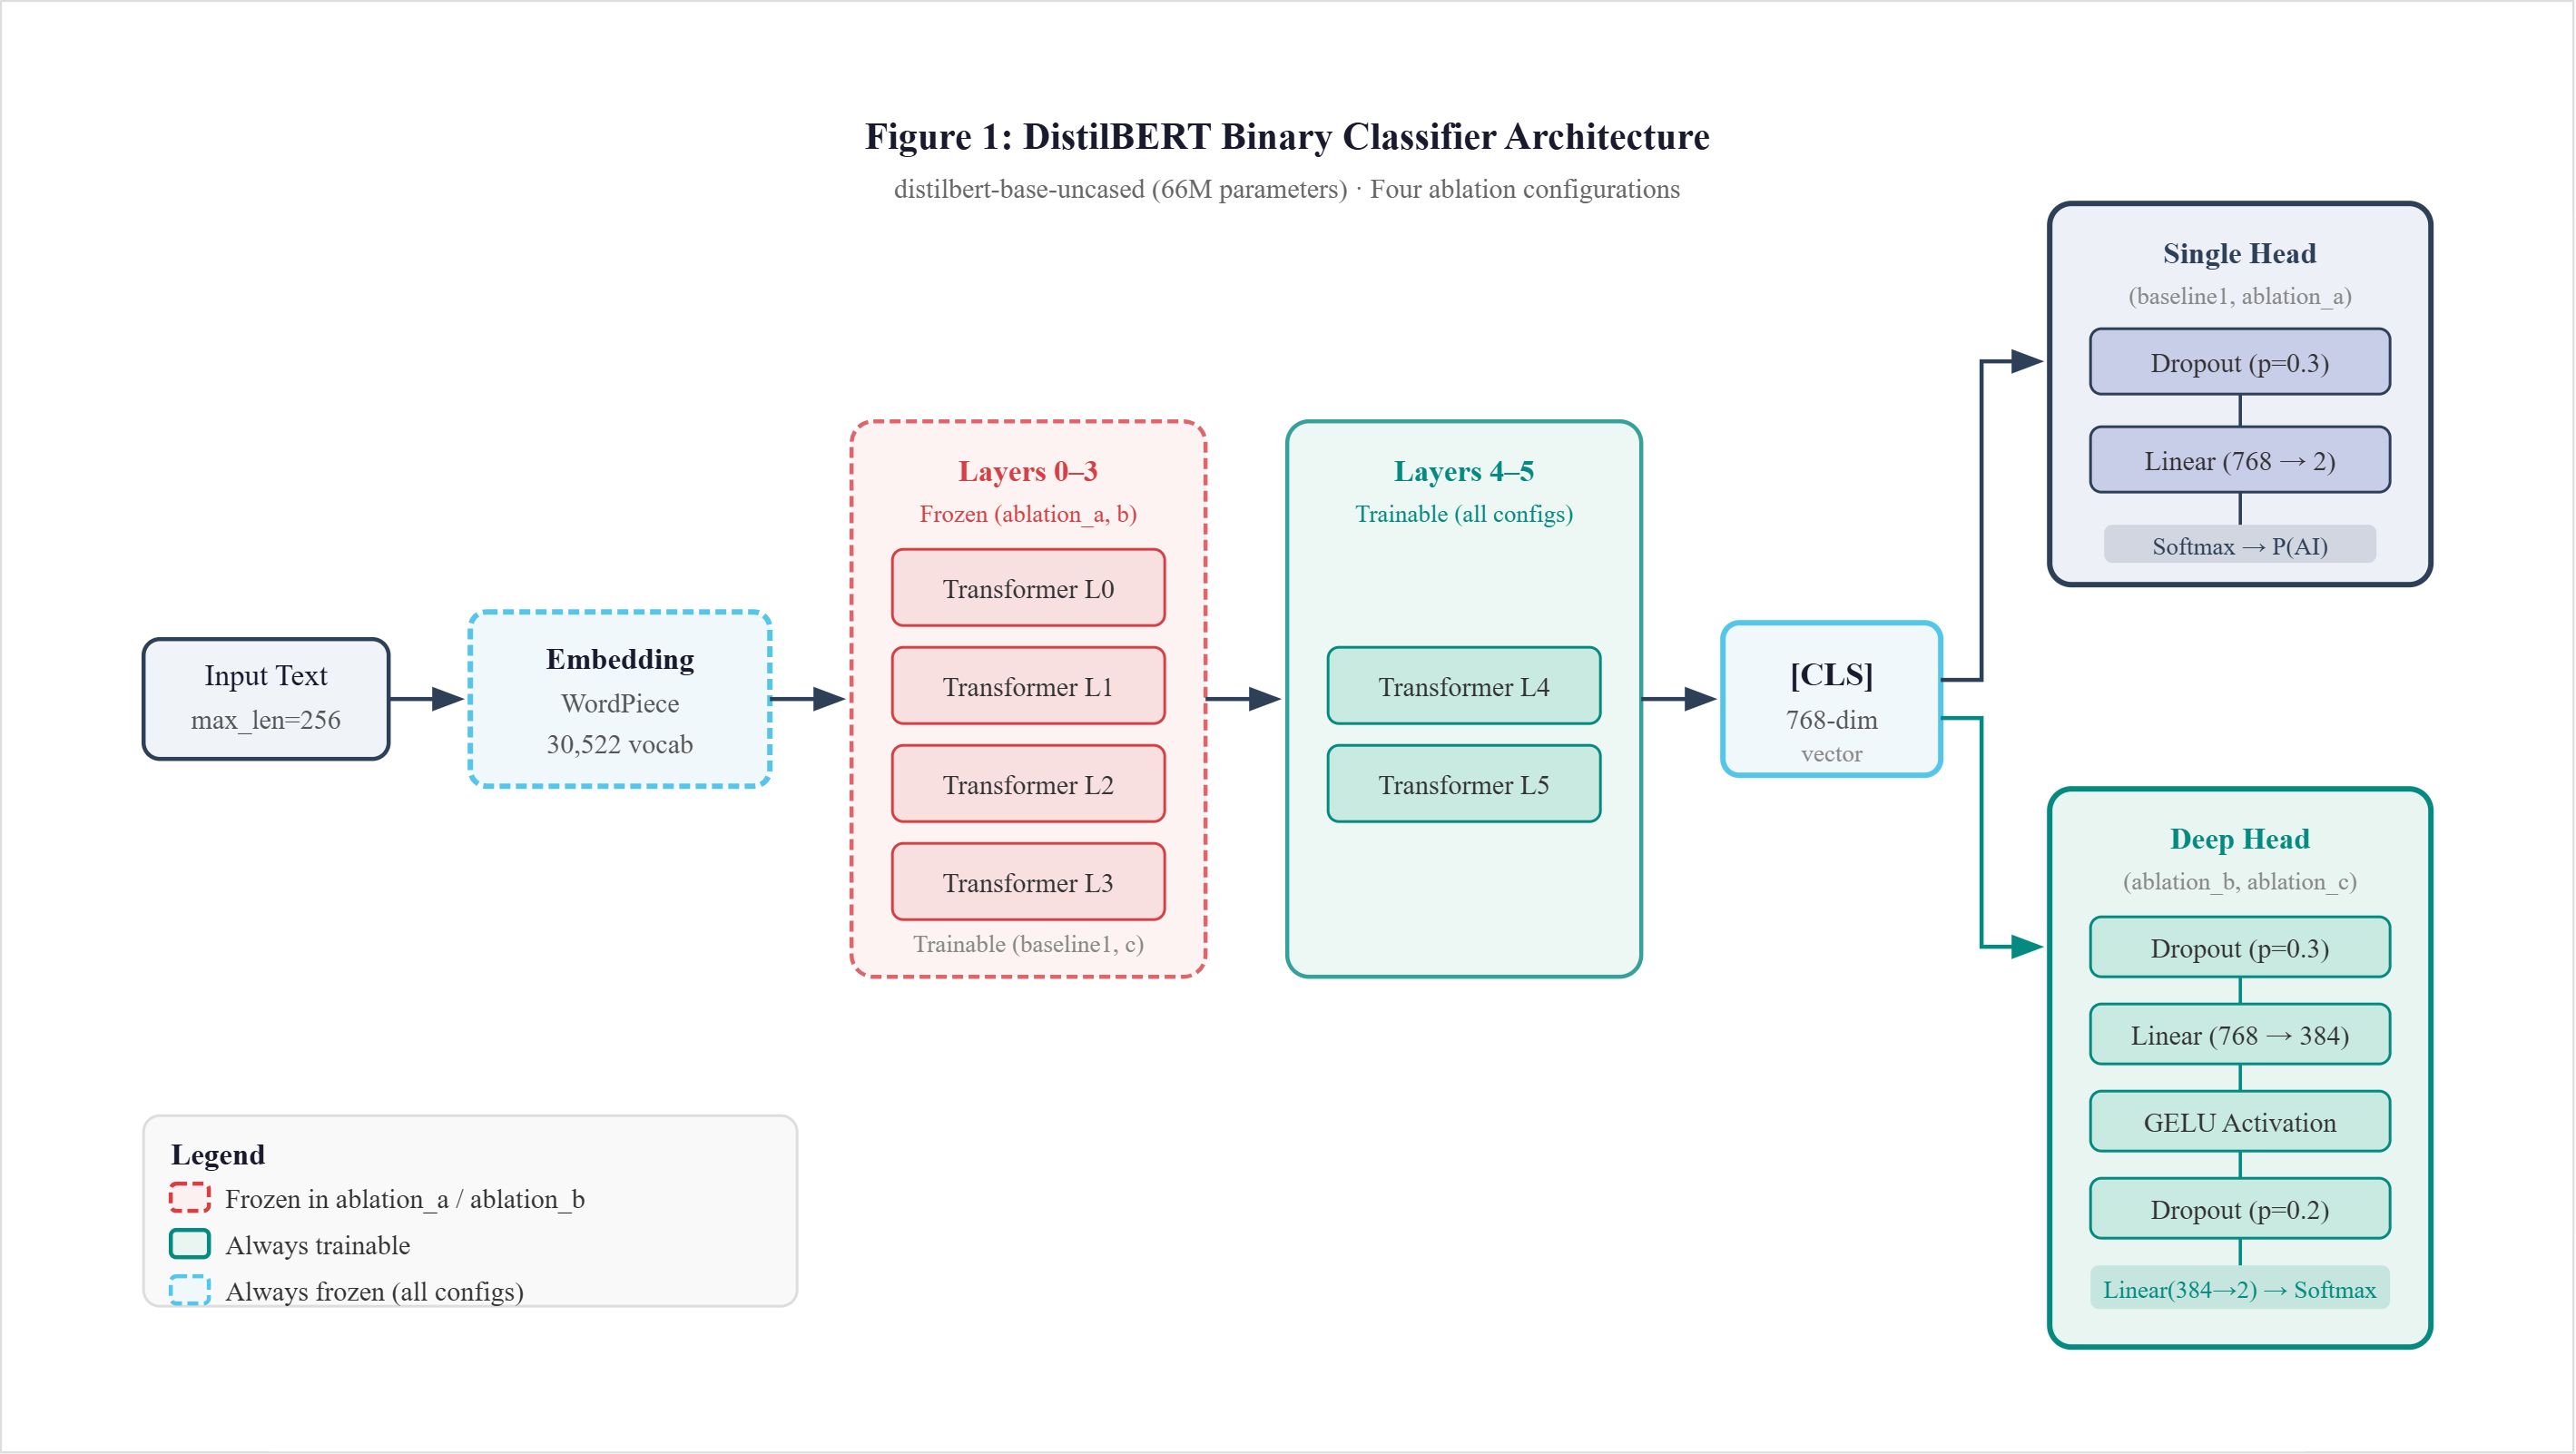
\includegraphics[width=\textwidth]{figures/figure1_architecture.png}
\caption{DistilBERT binary classifier architecture. The model
stacks a classification head atop the frozen \texttt{distilbert-base-uncased}
encoder. The [CLS] token's final hidden state (768-d) is passed to either
the single-layer head (\texttt{Dropout $\rightarrow$ Linear(768$\rightarrow$2)})
or the deep head (\texttt{Dropout $\rightarrow$ Linear(768$\rightarrow$384)
$\rightarrow$ GELU $\rightarrow$ Dropout $\rightarrow$ Linear(384$\rightarrow$2)}).
Embedding layers are always frozen; transformer layers 0--3 are optionally
frozen depending on ablation configuration.}
\label{fig:arch}
\end{figure*}

\textbf{Encoder backbone.} The base model is \texttt{distilbert-base-uncased}~\cite{sanh2019},
featuring 6~transformer layers, a hidden dimension of 768, 12~attention heads per layer,
and a WordPiece vocabulary of 30,522~entries. The total parameter count is approximately
66~million. We freeze the embedding layer during fine-tuning across all four configurations,
excluding its parameters from gradient computation. The classification head receives the
[CLS] token's final hidden state (a 768-dimensional vector) as the sequence representation.

\textbf{Classification head---single-layer variant.} This variant is used in
\texttt{baseline1} and \texttt{ablation\_a}:
\begin{center}
\small\texttt{Dropout(p=0.3) $\rightarrow$ Linear(768 $\rightarrow$ 2)}
\end{center}

\textbf{Classification head---deep variant.} This variant is used in
\texttt{ablation\_b} and \texttt{ablation\_c}:
\begin{center}
\small\texttt{Dropout(p=0.3) $\rightarrow$ Linear(768$\rightarrow$384)
$\rightarrow$ GELU $\rightarrow$ Dropout(p=0.2) $\rightarrow$ Linear(384$\rightarrow$2)}
\end{center}
The deep head adds one hidden layer with a GELU non-linearity and a second dropout stage.
The intermediate dimension of 384 creates a lightweight bottleneck at half the encoder's
hidden size. This additional non-linear projection provides the capacity to learn
attack-type-invariant decision boundaries from the encoder's representation, without
materially increasing parameter count or VRAM overhead relative to the encoder itself.

\textbf{Layer freezing strategy.} We study four configurations to isolate the independent
effects of head depth and encoder fine-tuning depth, summarised in Table~\ref{tab:configs}.

\begin{table}[t]
\caption{Ablation Configuration Summary}
\label{tab:configs}
\begin{center}
\small
\begin{tabular}{lllp{3.5cm}}
\toprule
\textbf{Config} & \textbf{Head} & \textbf{Frozen Layers} & \textbf{Description}\\
\midrule
\texttt{baseline1} & Single & 0 of 6 & Fully fine-tuned; shallow head\\
\texttt{ablation\_a} & Single & 0--3 (4 of 6) & Partially frozen; shallow head\\
\texttt{ablation\_b} & Deep & 0--3 (4 of 6) & Partially frozen; deep head; validation-selected\\
\texttt{ablation\_c} & Deep & 0 of 6 & Fully fine-tuned; deep head\\
\bottomrule
\end{tabular}
\end{center}
\end{table}

Freezing the lower four transformer layers preserves the general linguistic
representations learned during pre-training (syntactic and morphological);
the upper two layers are free to specialise toward the detection task.
This is a standard partial-freezing heuristic for fine-tuning on limited
data~\cite{goodfellow2016}, motivated by the constraint that lower layers
should not be overwritten by attack-specific signals that may not generalise.

\subsection{Seen / Held-Out Generator Split}\label{ssec:split}

Figure~\ref{fig:split} maps the split pipeline.
\begin{figure*}[t]
\centering
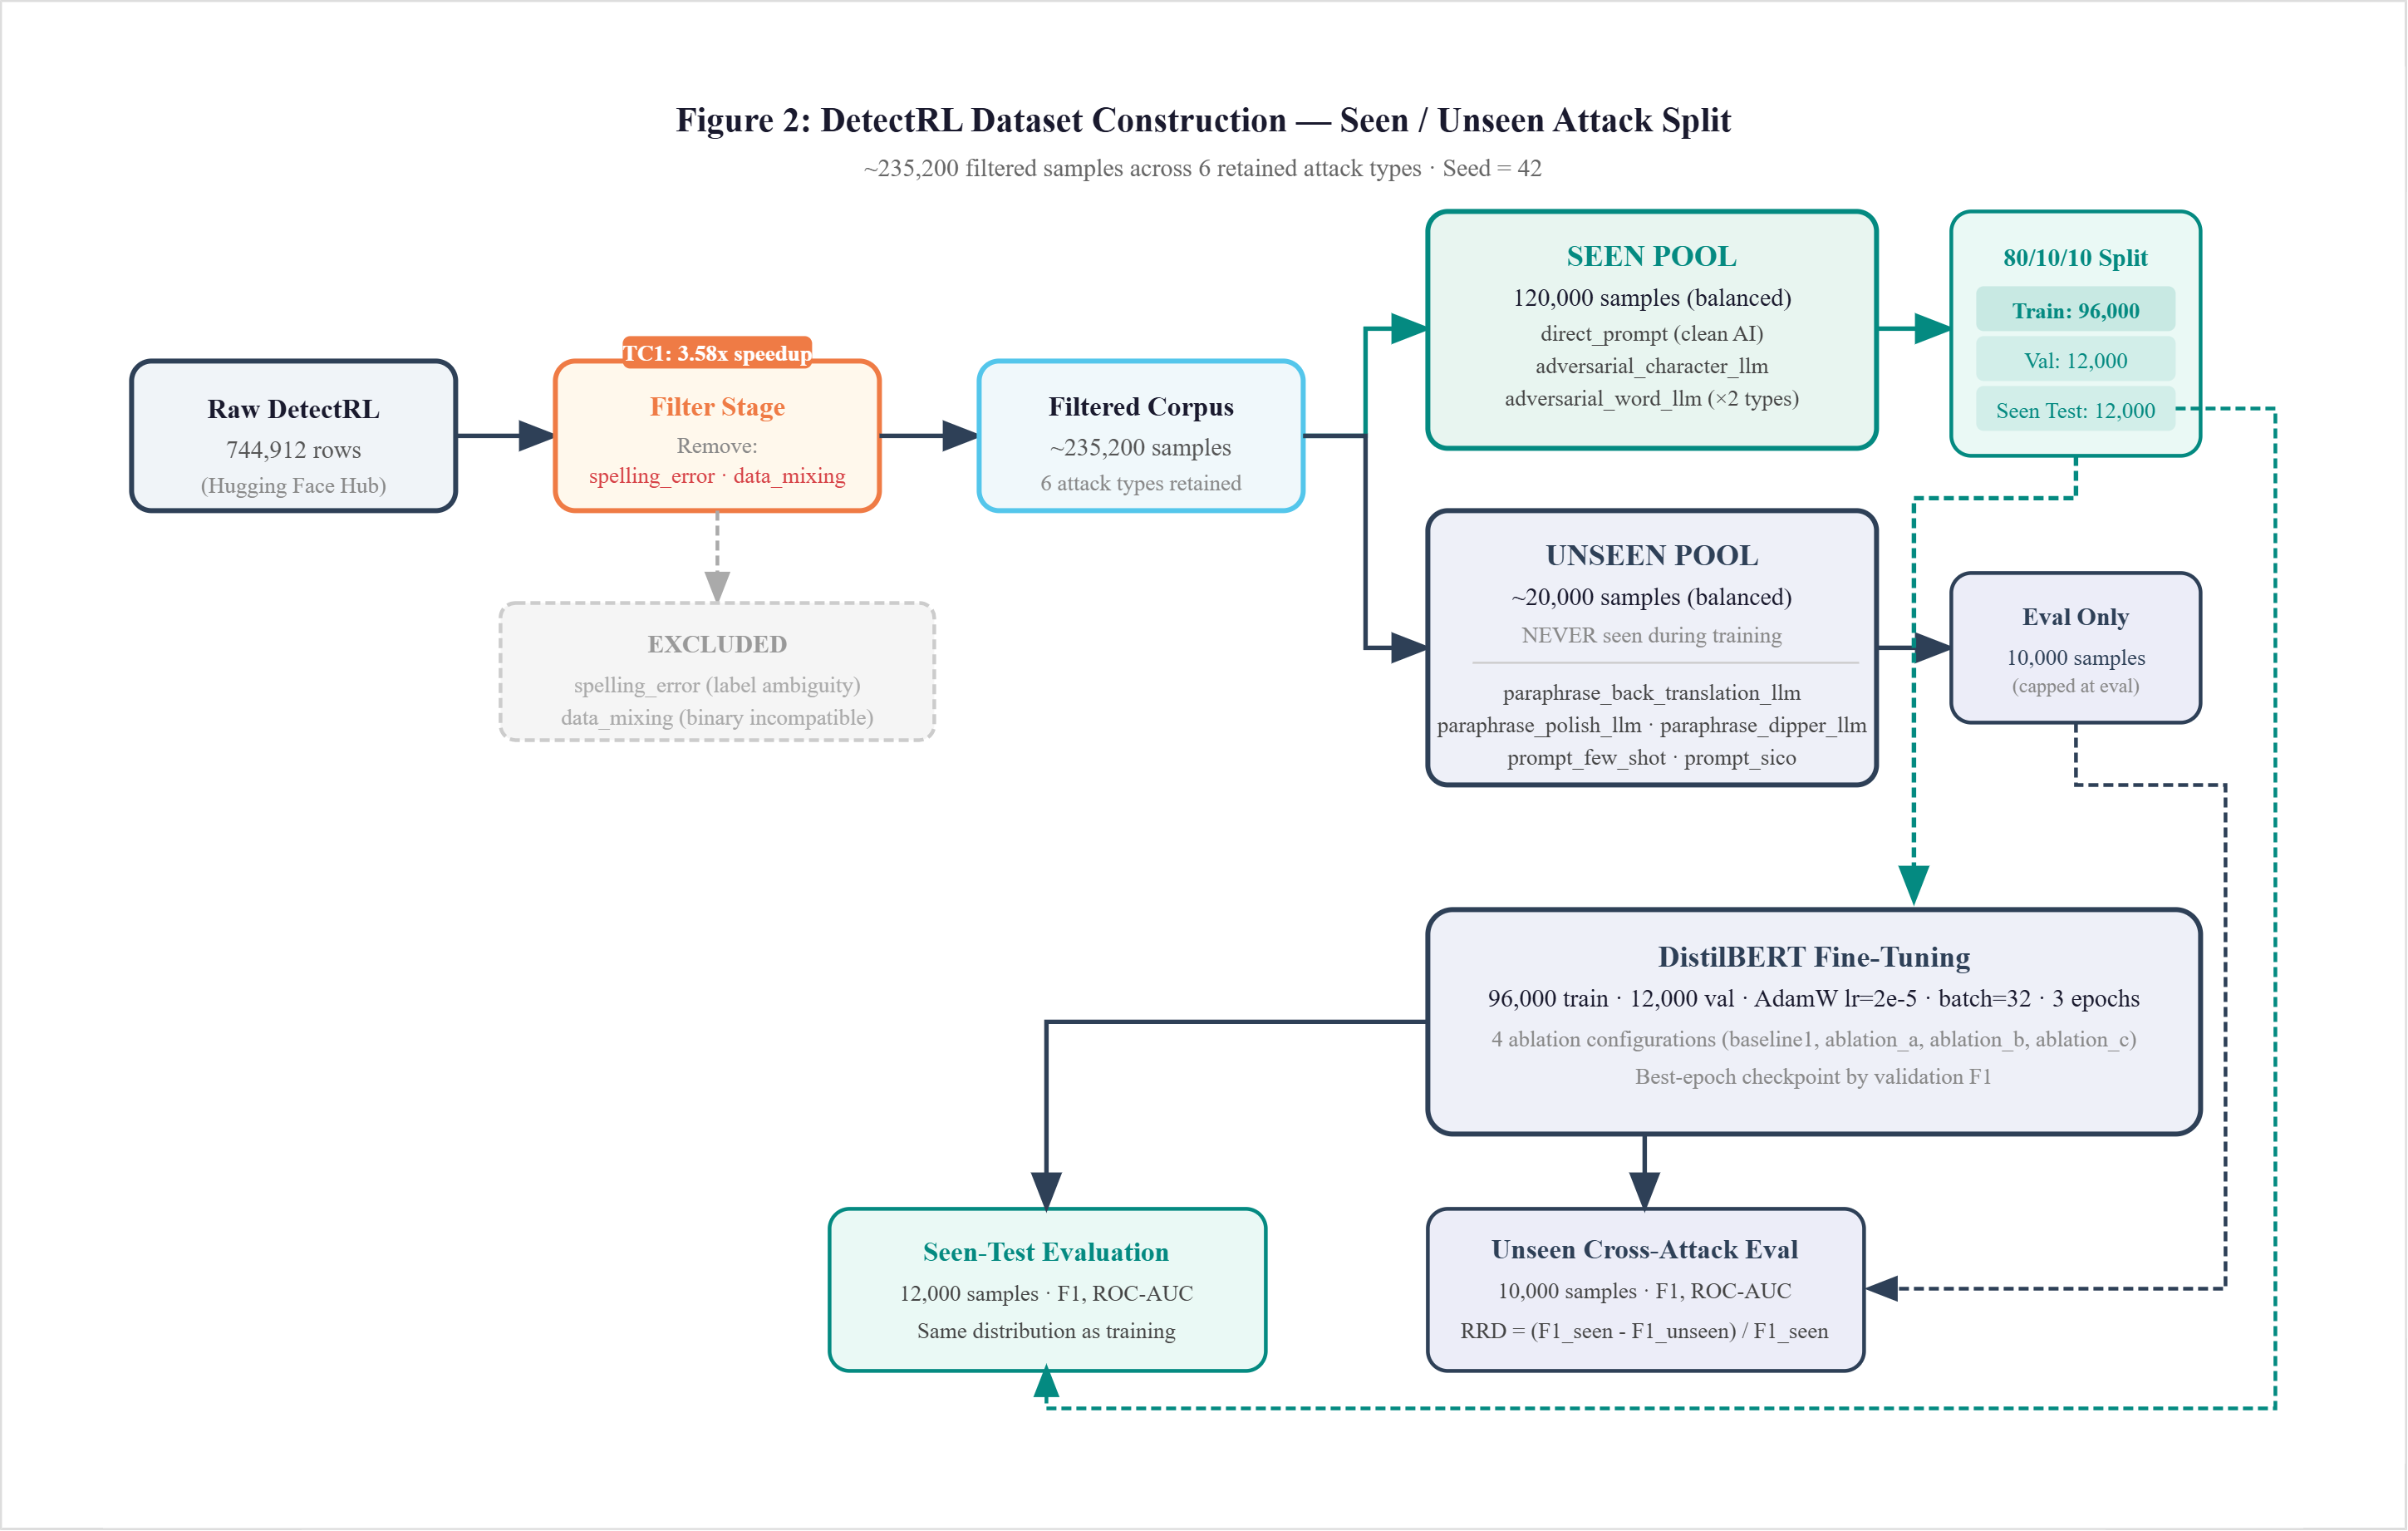
\includegraphics[width=\textwidth]{figures/figure2_split_pipeline.png}
\caption{Seen / held-out generator split pipeline. The RAID corpus is filtered
to retained domains, balanced into a 120,000-sample training pool from seen
generators, and evaluated on a separate held-out-generator pool. The
seen/held-out boundary separates source model families rather than attack
types; robustness is measured by comparing seen-generator test F1 against
held-out-generator F1.}
\label{fig:split}
\end{figure*}

The central experimental manipulation is the stratified seen/held-out split
over RAID generator families. The split maps RAID's \texttt{model} field into
three groups: seen generators, held-out generators, and excluded generators.

\textbf{Seen generator family.} The training and seen-test distribution uses
AI samples from \texttt{mpt}, \texttt{mistral}, \texttt{gpt2}, and
\texttt{llama-chat}, combined with human-written samples. These generators
provide broad coverage of open-source and older model families while leaving
stronger generators unseen during supervised fitting.

\textbf{Held-out generator family.} The held-out evaluation pool uses AI
samples from \texttt{gpt3}, \texttt{gpt4}, \texttt{chatgpt}, \texttt{cohere},
and \texttt{cohere-chat}, plus a balanced human subset. These samples are
withheld from training and validation and are used solely for generalisation
evaluation.

\textbf{Domain filtering.} We retain RAID rows from news, reddit, recipes,
poetry, and abstracts, which are sufficiently populated across the selected
generator families. The resulting split tests transfer across generator
families under RAID's adversarially augmented, multi-generator distribution.

\subsection{Training Protocol}

\textbf{Dataset construction.} We undersample RAID AI text from the seen-generator
pool and combine it with an equal number of human samples, yielding a balanced
training pool of 120,000~samples (60,000~human, 60,000~AI). Random permutation
with seed~42 splits this pool 80/10/10 into 96,000~training samples,
12,000~validation samples, and 12,000~seen-generator test samples. We construct
the held-out evaluation pool separately from withheld generators, balancing it to
20,000~samples (10,000~human, 10,000~AI) before applying the 10,000-sample
evaluation cap used by the training script.

\textbf{Tokenisation and data loading.} Samples are tokenised at
\texttt{max\_length=256} with padding and truncation. The primary training
pipeline performs tokenisation inside DataLoader worker processes so CPU
tokenisation overlaps with GPU training; the separate AMP timing experiment uses
the cached tensor workflow reported in the systems benchmark. We truncate to 256
(rather than DistilBERT's maximum of 512) to permit \texttt{batch\_size=32}
within 6~GB VRAM in the main ablation run.

\textbf{Optimiser and regularisation.} We train all configurations using the
AdamW optimiser at a learning rate of $2 \times 10^{-5}$ and weight decay of 0.01,
minimising CrossEntropyLoss. The positive-class posterior probability is thresholded at 0.5 (softmax decision threshold). Gradients are clipped
to a maximum L2~norm of 1.0 to prevent instability in early epochs. Each
configuration runs for 3~epochs. A global random seed of 42 is applied across
Python, NumPy, PyTorch, and CUDA for exact reproducibility.

\textbf{Checkpoint selection.} Validation F1 is computed post-epoch. The model
weights achieving the highest validation F1 across all epochs are saved and
used for all subsequent seen-test and held-out evaluations.

\subsection{Evaluation Metrics}

The primary evaluation metric is macro-averaged F1 (the arithmetic mean of the
per-class F1 scores). ROC-AUC serves as a threshold-free measure of overall
discriminative ability.
Accuracy, precision, and recall are reported as secondary diagnostics.
The primary generalisation metric is Relative Robustness
Degradation (RRD):
\begin{equation}
\text{RRD}(\%) = \frac{F1_{\text{seen}} - F1_{\text{held-out}}}{F1_{\text{seen}}} \times 100
\label{eq:rrd}
\end{equation}
Lower RRD indicates better held-out-generator generalisation. Following an interpretive heuristic (no established significance
criterion exists in the literature), an RRD below 5\%
indicates meaningful transfer of robustness; an RRD exceeding 10--15\% indicates
that generalisation has failed. This threshold is chosen descriptively to
contextualise observed RRD values and does not reflect formal significance
testing; we discuss this limitation in Section~\ref{ssec:limits}.

\subsection{Systems Optimisations (PP--AMP-I)}

Training four ablation configurations over 120,000~samples on a single RTX~4050 (6~GB)
requires deliberate systems engineering. We designed, implemented, and benchmarked
four optimisations:

\textbf{PP---Parallel multi-stage preprocessing.} Dataset filtering and pool
construction are parallelised across available CPU cores using Python's
multiprocessing pool. The recorded preprocessing benchmark reports a
3.58$\times$ speedup for parallel filtering over the sequential implementation.
For the RAID pipeline, the processed parquet files used by the DistilBERT
experiments are saved as \texttt{raid\_train\_pool.parquet} and
\texttt{raid\_test\_unseen.parquet}.

\textbf{DLO---Optimised DataLoader pipeline.} Parallel DataLoader workers overlap
CPU tokenisation and host-to-device transfer with GPU training. Combined with
\texttt{pin\_memory=True} and multi-worker prefetching, GPU starvation between
batches is reduced. GPU VRAM utilisation during the main training runs sits near
the full 6~GB dedicated capacity.

\textbf{AMP-T---Automatic Mixed Precision (AMP) training.} AMP training with
\texttt{GradScaler} is applied to \texttt{ablation\_b} (the validation-selected configuration)
with \texttt{batch\_size=128}---a 4$\times$ batch increase made feasible by the
reduced per-example VRAM footprint under FP16 activations. Under this regime,
\texttt{ablation\_b} completed 3~training epochs in 957.56~seconds at a peak VRAM
usage of 4,218.95~MB. Compared to the identical configuration under the baseline
32-batch training regime (3,180.47~seconds), this represents a 3.32$\times$
wall-clock speedup.

\textbf{AMP-I---AMP + inference-mode acceleration.} At inference time, combining
\texttt{torch.amp.autocast("cuda")} with \texttt{torch.inference\_mode()} eliminates
gradient bookkeeping. Benchmarked over 100~trials at batch size~32 with sequence
length~256, baseline FP32 latency was 183.75~ms/batch. The optimised configuration
achieved 84.07~ms/batch, representing a 54.25\% latency reduction and a throughput
of 380.64~samples/second.

% ---------------------------------------------------------------
\section{Experimental Setup}\label{sec:setup}

\subsection{Hardware and Software Environment}

DistilBERT experiments run on a Windows 10 workstation with an NVIDIA
RTX~4050 6~GB GPU, AMD Ryzen 5600X CPU (6 cores / 12 threads), 32~GB DDR4 RAM,
and NVMe SSD storage for parquet and tensor-cache I/O. The software stack is
Python~3.10.14, PyTorch~2.6.0 + CUDA~12.4, Transformers~5.6.2,
Datasets~4.8.4, scikit-learn~1.7.2, accelerate~1.13.0, NumPy~1.26.4, and
pandas~2.3.3. All experiments use \texttt{SEED=42} with
\texttt{torch.backends.cudnn.deterministic=True} and
\texttt{torch.backends.cudnn.benchmark=False} to ensure complete
reproducibility.

Regarding VRAM utilisation, the RTX~4050's 6~GB dedicated VRAM was fully
saturated during baseline training runs. The 16~GB of shared system memory
was accessed solely for DataLoader pinned-buffer staging---not for forward
or backward passes---meaning it did not bottleneck training throughput.

\subsection{DistilBERT Training Configuration}

Table~\ref{tab:hyperparams} summarises the training hyperparameters.

\begin{table}[t]
\caption{DistilBERT Training Hyperparameters}
\label{tab:hyperparams}
\begin{center}
\small
\begin{tabular}{ll}
\toprule
\textbf{Hyperparameter} & \textbf{Value}\\
\midrule
Base model             & \texttt{distilbert-base-uncased}\\
Max sequence length    & 256 tokens\\
Batch size (baseline)  & 32\\
Batch size (AMP-T)   & 128\\
Learning rate          & $2\times10^{-5}$\\
Optimiser              & AdamW\\
Weight decay           & 0.01\\
Gradient clip norm     & 1.0\\
Epochs                 & 3\\
Checkpoint criterion   & Best validation F1\\
Training set size      & 96,000 samples\\
Validation set size    & 12,000 samples\\
Seen test set size     & 12,000 samples\\
Unseen test set size   & 10,000 samples (capped from 20,000)\\
\bottomrule
\end{tabular}
\end{center}
\end{table}

The increase in batch size from 32 to 128 under AMP-T is a direct consequence
of Automatic Mixed Precision (AMP). FP16 activations halve per-example VRAM
consumption. Without this reduction, running \texttt{batch\_size=128} on the
RTX~4050 6~GB triggers an Out-Of-Memory (OOM) error. With AMP enabled, the
identical training loop peaks at 4,218.95~MB VRAM. This provides a
hardware-verified benefit beyond pure execution speed: AMP unlocks larger
batches that yield more stable gradient estimates.

\subsection{Efficiency Benchmarking Protocol}

Each optimisation case (PP--AMP-I) is benchmarked in isolation against an
unoptimised sequential baseline, following the per-stage instrumentation
strategy of Isenko et al.~\cite{isenko2022}:

\textbf{PP benchmark.} We compare a sequential filter run (single process,
GIL-bound, timed from parquet load to processed pool save) against a parallel
filter run (11~workers via Python multiprocessing pool). Both runs process
the full 744,912-row raw corpus and produce identical output files. Speedup
is calculated as sequential\_time / parallel\_time.

\textbf{DLO benchmark.} We measure GPU utilisation percentage via
\texttt{nvidia-smi} during training, comparing \texttt{num\_workers=0} against
\texttt{num\_workers=4} with \texttt{pin\_memory=True}. The pre-tokenisation
cache is active in both conditions to ensure the DataLoader's sole task is
tensor loading. This cleanly isolates the overlap benefit.

\textbf{AMP-T benchmark.} We compare wall-clock training time for
\texttt{ablation\_b} (3~epochs, batch=128) using AMP (\texttt{GradScaler} +
\texttt{autocast}) against the identical configuration's baseline non-AMP
time at batch=32 from \texttt{training\_times.json}. We record peak VRAM via
\texttt{torch.cuda.max\_memory\_allocated()}. This comparison reflects both
the precision speedup and the larger batch size made possible by AMP, as
these factors operate in tandem.

\textbf{AMP-I benchmark.} We conduct a 100-trial latency test (discarding a
10-trial warm-up) at batch=32 and seq\_len=256 using dummy input tensors.
The baseline is standard \texttt{torch.no\_grad()} FP32 inference. The
optimised condition uses \texttt{torch.inference\_mode()} combined with
\texttt{torch.amp.autocast("cuda")}. We report latency reduction percentage
and samples per second.

\subsection{GPT-2 XL Perplexity Reproduction Setup}
\label{ssec:reprosetup}

The GPT-2 XL Perplexity black-box pipeline was reproduced on a Kaggle
Tesla~T4 GPU (16~GB VRAM) using the official public repository. The black-box
run follows the \texttt{gpt3to4.sh} workflow with \texttt{gpt-j-6B} as both
sampling and scoring model over \texttt{xsum}, \texttt{writing}, and
\texttt{pubmed}, with source models \texttt{davinci},
\texttt{gpt-3.5-turbo}, and \texttt{gpt-4}. The representative white-box run
uses \texttt{squad}/\texttt{writing} with \texttt{gpt2-xl},
\texttt{opt-2.7b}, \texttt{gpt-neo-2.7B}, and \texttt{gpt-j-6B}.

\textbf{Intentional deviations.} The use of minimal black-box mode reduces
evaluation breadth compared to the full three-setting sweep, but preserves
the primary scoring configuration. Additionally, we skipped \texttt{gpt-neox-20B}
due to Kaggle resource constraints. These deviations preclude reproduction
of the 5-model AUROC aggregate; therefore, only the ChatGPT/GPT-4 aggregate
is compared to the original paper target. All applied patches (tokeniser
compatibility fixes, low-memory model loading, disk preflight checks, and
session-resume logic) serve as operational safeguards and do not alter the
fundamental detection criterion.

\textbf{Tokeniser compatibility patch.} The official GPT-2 XL Perplexity
repository loads scoring-model tokenisers without configuring the padding
token. Decoder-only causal LLMs (like \texttt{gpt-j-6B} and \texttt{gpt2-xl})
do not define a \texttt{pad\_token} by default, causing a \texttt{ValueError}
when padding batched inputs. We applied two targeted fixes. First, a
\texttt{pad\_token is None} guard assigns the end-of-sequence token as the
padding sentinel (\texttt{tokenizer.pad\_token = tokenizer.eos\_token})---a
standard Hugging Face workaround for GPT-family models. Second, we explicitly
enforce right-padding (\texttt{tokenizer.padding\_side = "right"}) to guarantee
correct attention-mask alignment. Neither fix alters the scoring criterion.
The detection signal remains computed from per-token log-probabilities on the
non-padded prefix, while the attention mask correctly excludes padding positions
from the model's receptive field during inference.

\subsection{GPT-2 XL Perplexity RAID Extension Setup}
\label{ssec:raidsetup}

The RAID adversarial evaluation of GPT-2 XL Perplexity was run locally with
PyTorch~2.6.0 + CUDA~12.4 and 4-bit NF4 BitsAndBytes quantisation. We use
\texttt{gpt-j-6B} as the sampling model and evaluate \texttt{gpt-j-6B} and
\texttt{gpt2-xl} as scoring models, both quantised to NF4. The RAID homoglyph
and paraphrase subsets each contain 1,000 balanced samples (500 human / 500 AI,
seed=42). We use 2,500 Monte Carlo (MC) samples, bootstrap 95\% confidence intervals (CIs) with 1,000 iterations,
and two-sided empirical $p$-values.

We selected the Monte Carlo (MC) sample count of 2,500 via ablation on a
200-sample calibration set from RAID. AUROC stability was evaluated across
$MC \in \{1,000; 2,000; 5,000; 10,000\}$. The 2,500 threshold marked the
point of diminishing returns on AUROC improvement relative to runtime cost.
Because the two RAID subsets are independent, non-overlapping samples, the
bootstrap difference test specifically captures population-level
distributional differences between attack conditions rather than
within-document paired effects.

% ---------------------------------------------------------------
\section{Results}\label{sec:results}

\subsection{Reproduced Baseline Results}\label{ssec:reproduced}

We reproduce the GPT-2 XL Perplexity~\cite{bao2024} black-box pipeline using
the official repository on a Kaggle Tesla~T4 GPU. The reproduction targets
the ChatGPT/GPT-4 generations aggregate AUROC (paper target: 0.9338). The
5-model aggregate is excluded following the intentional omission of
\texttt{gpt-neox-20B}.

\subsubsection{Black-Box Per-Setting Results}

\begin{table}[t]
\caption{GPT-2 XL Perplexity Black-Box AUROC and PR-AUC Per Setting}
\label{tab:blackbox}
\begin{center}
\small
\begin{tabular}{lcc}
\toprule
\textbf{Setting (Dataset / Source Model)} & \textbf{AUROC} & \textbf{PR-AUC}\\
\midrule
xsum / davinci          & 0.9333 & 0.9332\\
xsum / gpt-3.5-turbo    & 0.9920 & 0.9937\\
xsum / gpt-4            & 0.9160 & 0.9137\\
writing / davinci       & 0.9572 & 0.9526\\
writing / gpt-3.5-turbo & 0.9966 & 0.9975\\
writing / gpt-4         & 0.9762 & 0.9792\\
pubmed / davinci        & 0.6663 & 0.6697\\
pubmed / gpt-3.5-turbo  & 0.9039 & 0.8883\\
pubmed / gpt-4          & 0.8376 & 0.8203\\
\bottomrule
\end{tabular}
\end{center}
\end{table}

\textbf{Observations (Table~\ref{tab:blackbox}).} Performance is heavily domain-dependent. The
\texttt{writing} dataset yields the highest AUROC across all source models
(0.9762--0.9966), indicating that creative writing prompts elicit the most
distinctive AI generation patterns. Conversely, the \texttt{pubmed} domain
exhibits a sharp drop for the \texttt{davinci} model (AUROC 0.6663). This is
attributable to biomedical text's compact, high-information-density style,
which places it outside the conditional probability distribution GPT-2 XL Perplexity
was calibrated on. Furthermore, GPT-4 generated text is consistently harder to
detect than GPT-3.5 and \texttt{davinci} text across all three datasets. This
aligns with the documented trend that frontier models produce increasingly
human-indistinguishable text.

\subsubsection{Paper vs.\ Reproduced Aggregate Comparison}

The reproduced ChatGPT/GPT-4 aggregate AUROC is 0.9370, compared with the
original paper target of 0.9338 ($+0.0032$). The original 5-model aggregate
(0.9887) is not reproduced because \texttt{gpt-neox-20B} is excluded under the
resource constraint described above. The small ChatGPT/GPT-4 difference falls
within stochastic variation expected from Monte Carlo sampling and does not
represent a systematic improvement; it indicates implementation fidelity.

\subsubsection{White-Box Representative Results}

White-box representative checks provide secondary confirmation that the
pipeline implementation is faithful: \texttt{squad}/\texttt{gpt-j-6B} reaches
0.9852 AUROC, while \texttt{writing} runs across \texttt{gpt2-xl},
\texttt{opt-2.7b}, \texttt{gpt-neo-2.7B}, and \texttt{gpt-j-6B} fall in the
0.9971--0.9982 AUROC range.

\subsection{Additional Experiment Results}\label{ssec:additional}

This section details the primary DistilBERT held-out-generator generalisation
ablation study, followed by the systems optimisation benchmarks and
the GPT-2 XL Perplexity RAID adversarial evaluation.

\subsubsection{DistilBERT Ablation Study: Held-Out-Generator Generalisation}

\begin{table*}[t]
\caption{Per-Ablation Performance --- Seen-Generator Test Split and Held-Out-Generator Split}
\label{tab:ablation}
\begin{center}
\footnotesize
\begin{tabular}{lcccccc}
\toprule
\textbf{Config} & \textbf{Best Val F1} & \textbf{Seen F1} & \textbf{Seen ROC-AUC} & \textbf{Held-out F1} & \textbf{Held-out ROC-AUC} & \textbf{RRD (\%)}\\
\midrule
\texttt{baseline1}               & 0.9442 & 0.9238 & 0.9879 & 0.9135 & 0.9733 & \textbf{1.11}\\
\texttt{ablation\_a}             & 0.9421 & 0.9409 & 0.9900 & 0.9267 & 0.9775 & \textbf{1.51}\\
\texttt{ablation\_b} (val-selected)  & \textbf{0.9488} & \textbf{0.9481} & 0.9908 & 0.9184 & 0.9743 & 3.13\\
\texttt{ablation\_c}             & 0.9484 & 0.9472 & \textbf{0.9923} & \textbf{0.9263} & \textbf{0.9790} & 2.21\\
\bottomrule
\multicolumn{7}{l}{\footnotesize All metrics from single-seed evaluation (seed=42); reported for directional comparison only.}\\
\end{tabular}
\end{center}
\end{table*}

\begin{table*}[t]
\caption{Full Diagnostic Metrics --- Seen-Generator and Held-Out-Generator Splits}
\label{tab:diagnostic}
\begin{center}
\footnotesize
\begin{tabular}{lcccccccc}
\toprule
\textbf{Config} & \textbf{S.Acc} & \textbf{S.Prec} & \textbf{S.Rec} & \textbf{S.F1} & \textbf{H.Acc} & \textbf{H.Prec} & \textbf{H.Rec} & \textbf{H.F1}\\
\midrule
\texttt{baseline1}  & 0.9195 & 0.8768 & 0.9762 & 0.9238 & 0.9110 & 0.8889 & 0.9394 & 0.9135\\
\texttt{ablation\_a}& 0.9393 & 0.9177 & 0.9652 & 0.9409 & 0.9269 & 0.9294 & 0.9240 & 0.9267\\
\texttt{ablation\_b}& 0.9474 & 0.9352 & 0.9615 & 0.9481 & 0.9205 & 0.9433 & 0.8948 & 0.9184\\
\texttt{ablation\_c}& 0.9453 & 0.9157 & 0.9810 & 0.9472 & 0.9261 & 0.9243 & 0.9282 & 0.9263\\
\bottomrule
\multicolumn{9}{l}{\footnotesize S.~= Seen-generator split; H.~= Held-out-generator split; Acc~= Accuracy; Prec~= Precision; Rec~= Recall.}
\end{tabular}
\end{center}
\end{table*}

\begin{table}[t]
\caption{Wall-Clock Training Times and Trainable Parameter Counts (3 epochs, batch=32, RTX 4050 6 GB)}
\label{tab:wallclock}
\begin{center}
\footnotesize
\begin{tabular}{lllrr}
\toprule
\textbf{Config} & \textbf{Head} & \textbf{Frozen} & \textbf{Params} & \textbf{Time (s)}\\
\midrule
\texttt{baseline1}  & Single & 0 of 6 & 42,514,946 & 5,293.68\\
\texttt{ablation\_a}& Single & 4 of 6 & 14,172,674 & 3,183.73\\
\texttt{ablation\_b}& Deep   & 4 of 6 & 14,467,202 & 3,180.47\\
\texttt{ablation\_c}& Deep   & 0 of 6 & 42,809,474 & 5,295.62\\
\bottomrule
\multicolumn{5}{l}{\footnotesize Counts derived from DistilBERT-base-uncased architecture.}
\end{tabular}
\end{center}
\end{table}

\begin{table}[t]
\caption{Confusion Matrices for \texttt{ablation\_c}}
\label{tab:conf_seen}
\begin{center}
\small
\begin{tabular}{llcc}
\toprule
\textbf{Split} & \textbf{Actual} & \textbf{Pred: Human} & \textbf{Pred: AI}\\
\midrule
\multirow{2}{*}{Seen} & Human & TN = 5,461 & FP = 539\\
 & AI & FN = 114 & TP = 5,886\\
\midrule
\multirow{2}{*}{Held-out} & Human & TN = 4,622 & FP = 378\\
 & AI & FN = 359 & TP = 4,641\\
\bottomrule
\end{tabular}

\vspace{4pt}
\footnotesize Seen split: $N=12{,}000$; held-out split: $N=10{,}000$. Both are balanced 50/50.
\end{center}
\end{table}

Validation and ablation metrics are reported in Tables~\ref{tab:ablation}
and~\ref{tab:diagnostic}. Held-out-generator generalisation holds across all
four configurations.
Held-out F1 ranges from 0.914 to 0.927 (Table~\ref{tab:ablation}), and RRD values span 1.1\% to
3.1\%---well below the 5\% interpretive threshold described following
\eqref{eq:rrd}. This answers RQ1 positively for the RAID generator split:
representations learned from adversarially augmented seen-generator data
transfer meaningfully to withheld generator families.

Head depth modestly raises seen-test precision at a cost to
held-out-generator transfer (Table~\ref{tab:diagnostic}). Comparing \texttt{ablation\_a} (single head,
freeze=4) against \texttt{ablation\_b} (deep head, freeze=4) shows that
seen F1 increases by $+$0.72~pp while unseen F1 decreases by $-$0.83~pp.
This raises RRD from 1.51\% to 3.13\%. The deep head extracts greater
in-distribution signal from the partially-frozen encoder, but this
specialisation exacts a measurable cost on held-out performance.

\texttt{ablation\_c} (deep head, fully unfrozen) achieves the strongest
threshold-free held-out performance. It records the highest seen ROC-AUC
(0.9923), the highest held-out ROC-AUC (0.9790), and a held-out F1 of
0.9263, effectively tied with \texttt{ablation\_a}'s 0.9267. Its moderate
RRD of 2.21\% is higher than \texttt{baseline1} and \texttt{ablation\_a},
but lower than \texttt{ablation\_b}. This suggests that full encoder
fine-tuning improves discriminative ranking while not necessarily minimising
relative degradation.

The confusion matrix (Table~\ref{tab:conf_seen}) reveals a critical
asymmetry across splits. On the seen split, the model
exhibits a strong recall bias: it misses only 114~AI samples (1.9\% of AI)
but misclassifies 539~human samples as AI (9.0\% of human). On the unseen
split, this asymmetry partially corrects. False negatives rise to 359 (7.2\%
of AI) and false positives fall to 378 (7.6\% of human), indicating the model
behaves more conservatively under out-of-distribution attack types. The
near-equal FN/FP balance on the unseen split (359 vs.\ 378) serves as a
positive generalisation signal, suggesting the decision boundary shifts
coherently rather than collapsing into a trivial class bias.

Training time (Table~\ref{tab:wallclock}) scales entirely with the number of trainable parameters
rather than classification head depth. Fully unfrozen configurations
(\texttt{baseline1}, \texttt{ablation\_c}) require approximately 5,294~seconds.
Partially frozen configurations (\texttt{ablation\_a}, \texttt{ablation\_b})
require approximately 3,182~seconds. The four additional unfrozen transformer
layers drive this 1.66$\times$ overhead.

\subsubsection{Efficiency Optimisation Benchmark Results}

Figure~\ref{fig:efficiency} and Table~\ref{tab:efficiency_benchmarks} summarise the per-stage
optimisation gains.

\begin{figure}[t]
\centering
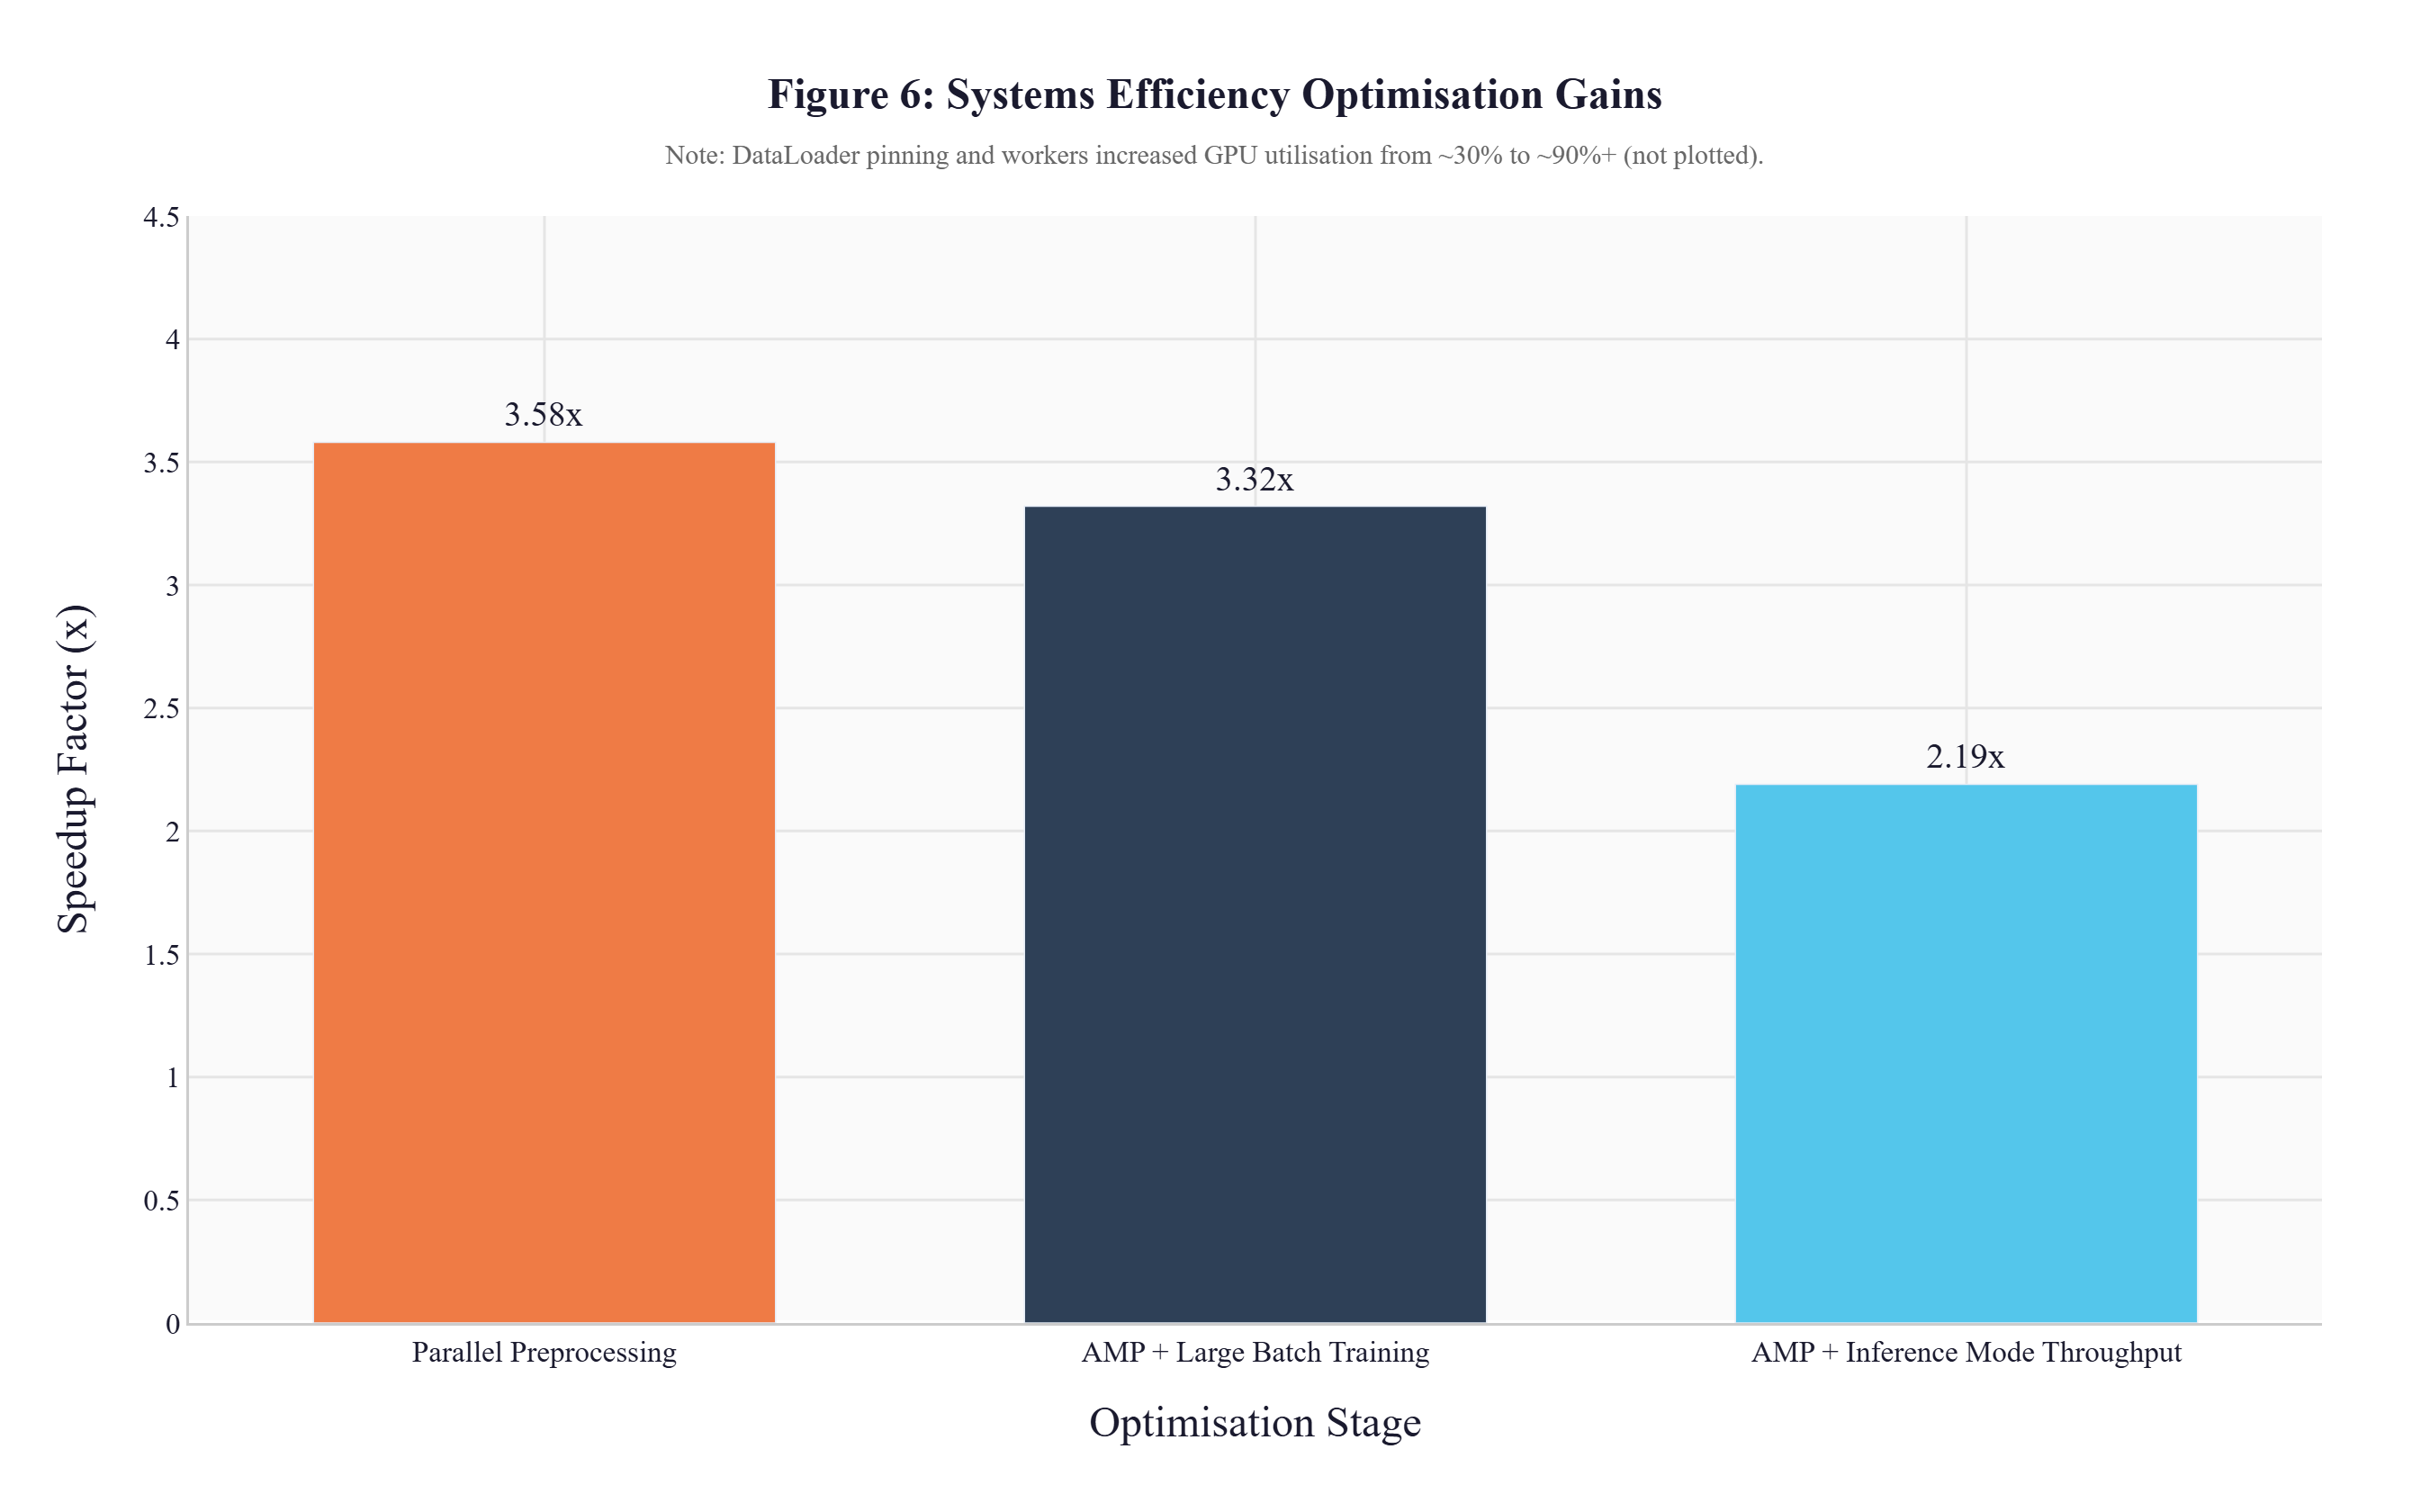
\includegraphics[width=\columnwidth]{figures/figure3_efficiency_speedup.png}
\caption{Pipeline optimisation gains by stage. Bar chart
of multiplicative speedup factors for parallel preprocessing (3.58$\times$),
AMP training with a larger batch (3.32$\times$), and AMP inference mode
(2.19$\times$ throughput). The optimised DataLoader increased GPU utilisation from
$\sim$30--50\% to $\sim$80--90\%+ but is not expressed as a speedup factor.
All gains were measured on the same RTX~4050 6~GB hardware.}
\label{fig:efficiency}
\end{figure}

\begin{table*}[t]
\caption{Efficiency Benchmark Results Summary}
\label{tab:efficiency_benchmarks}
\begin{center}
\footnotesize
\begin{tabular}{llrrl}
\toprule
\textbf{Stage} & \textbf{Metric} & \textbf{Baseline} & \textbf{Optimised} & \textbf{Gain}\\
\midrule
PP --- Parallel preprocessing & Filter time (s)   & 31.83 & 8.89            & \textbf{3.58$\times$ speedup}\\
PP --- Parallel preprocessing & Workers           & 1 (GIL-bound) & 11         & ---\\
DLO --- Optimised DataLoader   & GPU utilisation   & $\sim$30--50\% & $\sim$80--90\%+ & $\sim$1.6--3.0$\times$ duty cycle improvement\\
AMP-T --- AMP + large batch      & Train time, s     & 3,180.47 (batch=32) & 957.56 (batch=128) & \textbf{3.32$\times$ speedup}\\
AMP-T --- AMP + large batch      & Peak VRAM (MB)    & $>$8,000 (OOM at batch=128)       & \textbf{4,218.95} & $-$47.3\% VRAM\\
AMP-I --- AMP + inference mode   & Batch latency (ms)& 183.75 & \textbf{84.07} & \textbf{54.25\% reduction}\\
AMP-I --- AMP + inference mode   & Throughput (samp/s) & $\sim$174 & \textbf{380.64} & 2.19$\times$ throughput\\
\bottomrule
\end{tabular}
\end{center}
\end{table*}

\textbf{AMP-T causal detail.} The AMP-T speedup (3.32$\times$) and batch size
increase (32$\rightarrow$128) are causally linked. AMP's FP16 activations
halve per-example VRAM consumption, freeing sufficient headroom to run
\texttt{batch\_size=128} on the 6~GB RTX~4050 without triggering an OOM
error. Running \texttt{batch\_size=128} in FP32 causes an immediate crash.
With AMP enabled, the identical loop peaks at 4,218.95~MB, sitting 47\%
below the OOM threshold. The composite benefit---AMP precision combined
with a 4$\times$ larger batch requiring fewer gradient steps per epoch---produces
the 3.32$\times$ wall-clock speedup. On this specific hardware, AMP's memory
efficiency yields a more practically significant benefit than its raw
compute acceleration.

\subsubsection{GPT-2 XL Perplexity RAID Adversarial Evaluation}

Figure~\ref{fig:raid_auroc} and Table~\ref{tab:raid} present GPT-2 XL Perplexity's
AUROC on RAID adversarial subsets.

\begin{figure}[t]
\centering
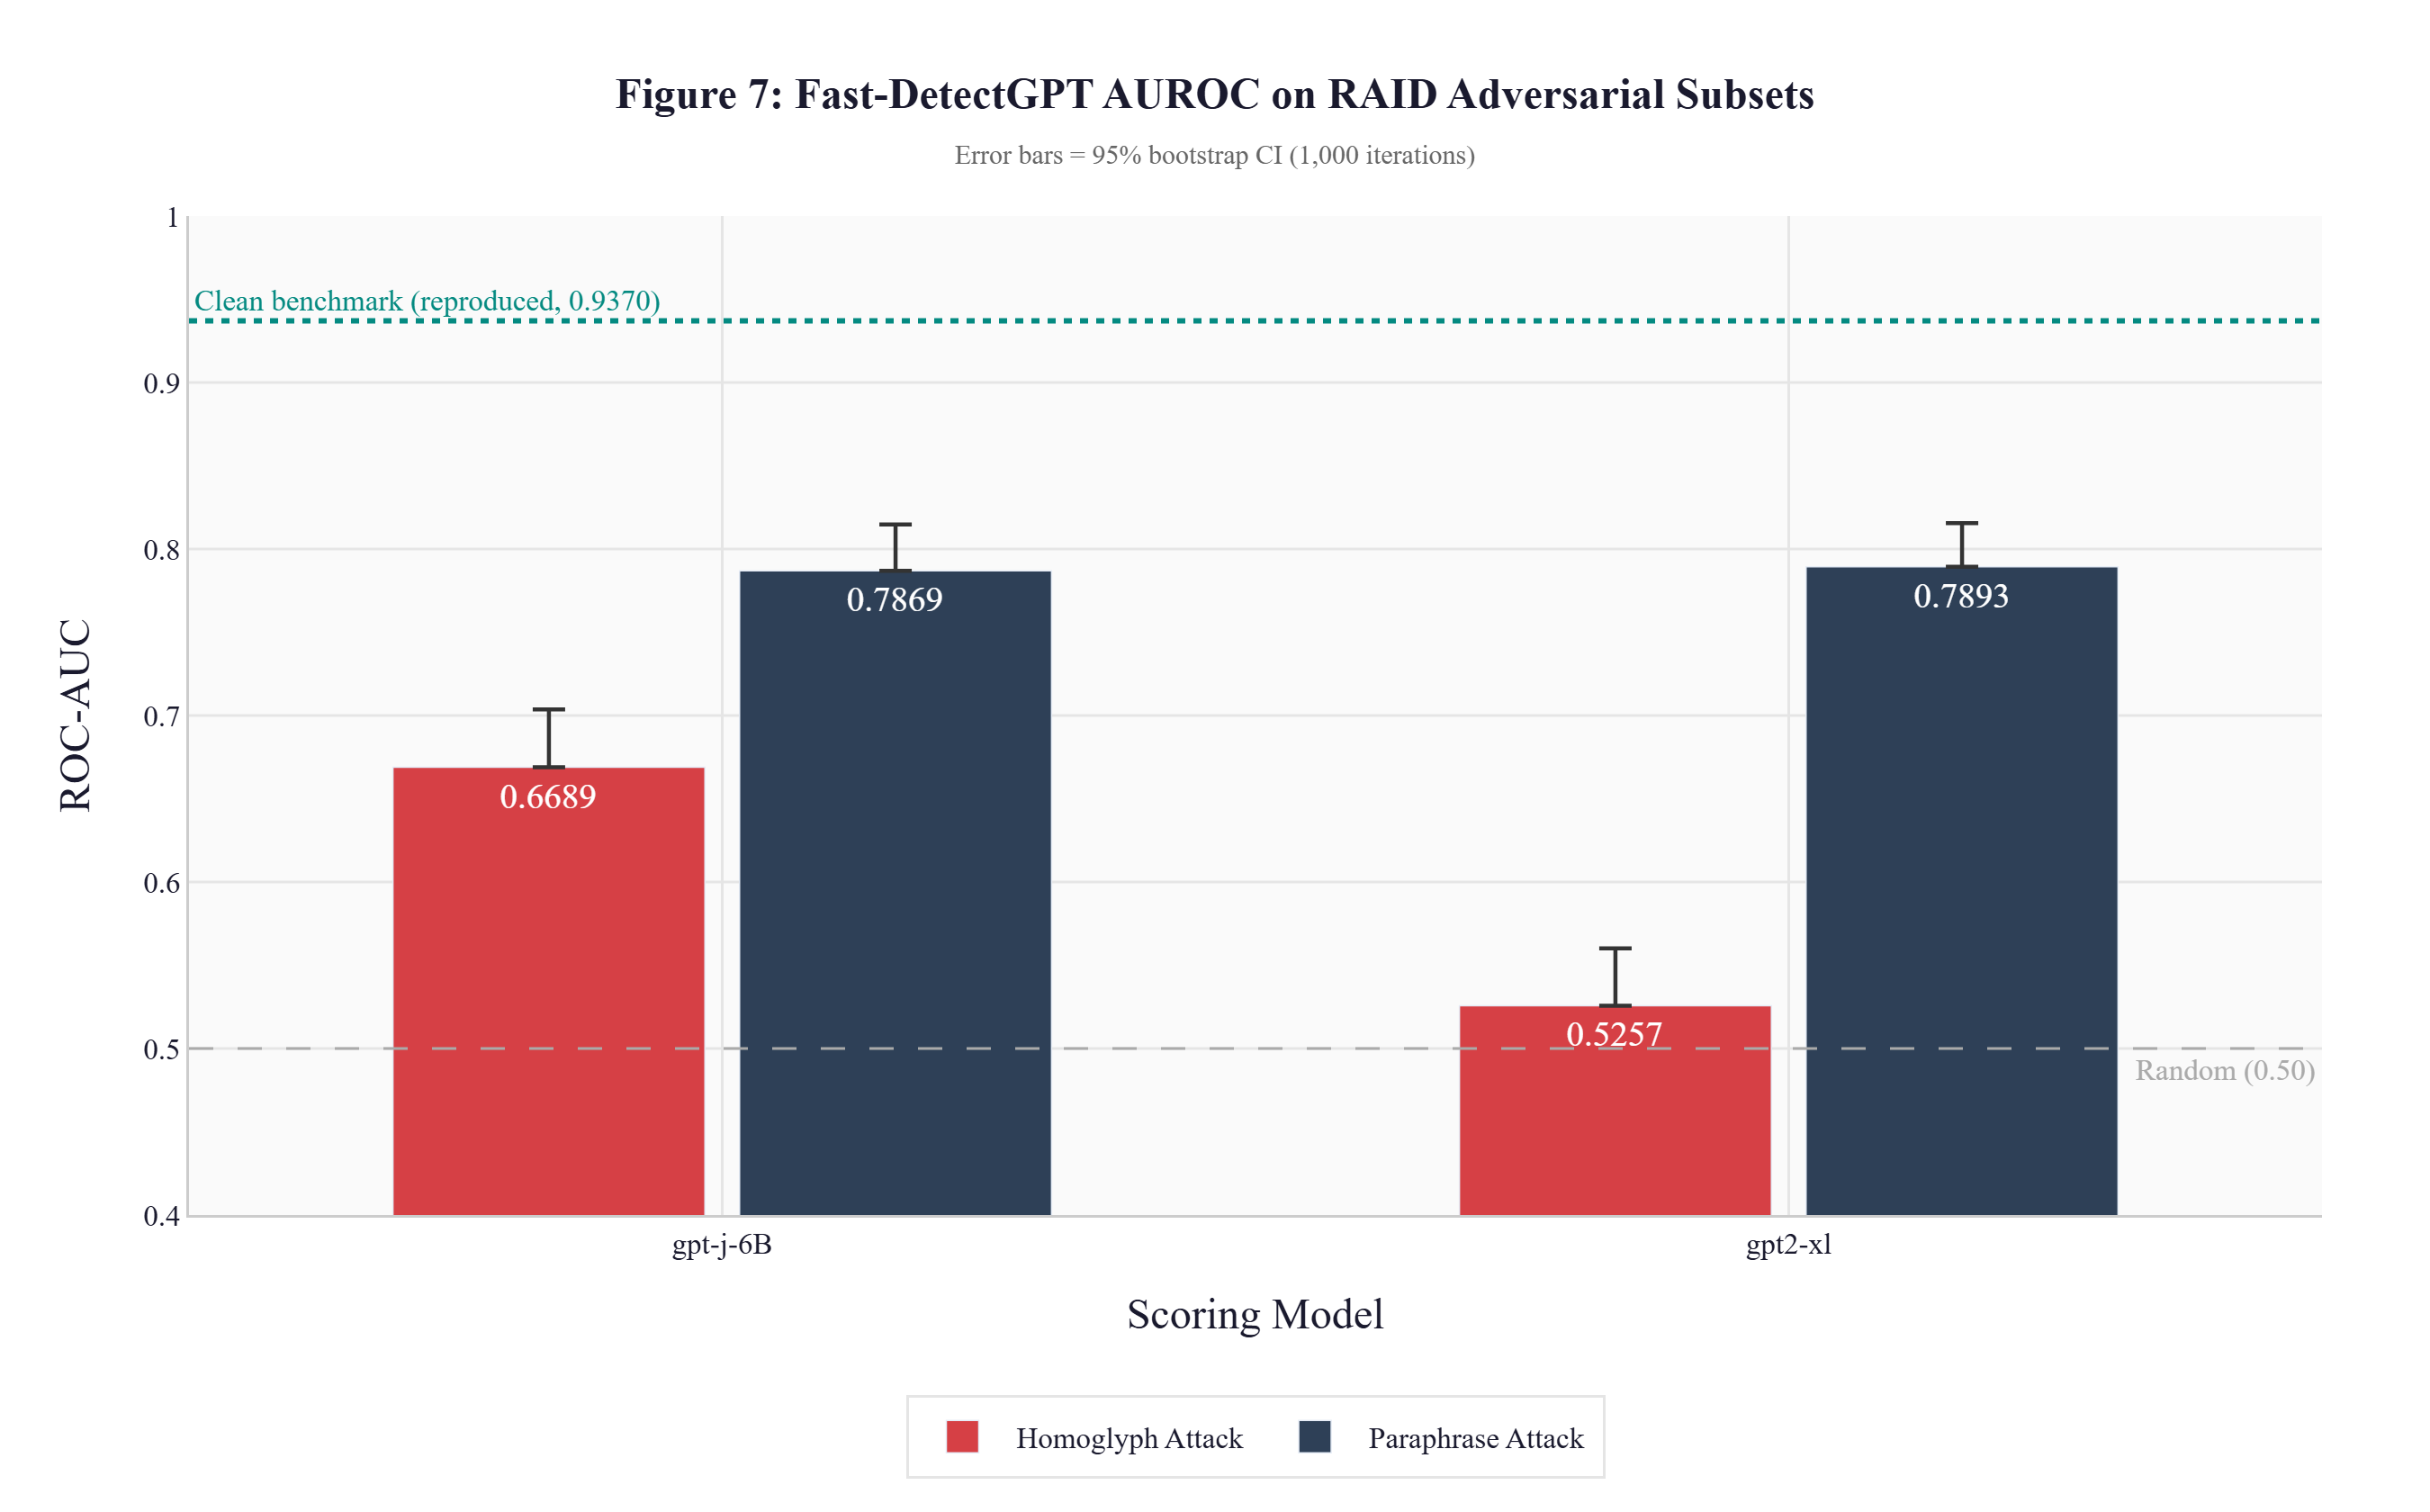
\includegraphics[width=\columnwidth]{figures/figure4_raid_auroc_comparison.png}
\caption{GPT-2 XL Perplexity AUROC on RAID adversarial subsets. Paraphrase AUROC
is near-identical across scorers ($\sim$0.787--0.789), while Homoglyph
AUROC diverges sharply by scorer size (gpt-j-6B: 0.6689 vs.\ gpt2-xl:
0.5257), indicating that scorer capacity specifically aids robustness to
character-level Unicode corruption. The clean benchmark reference line
(0.9370) highlights the magnitude of adversarial degradation.}
\label{fig:raid_auroc}
\end{figure}

\begin{table*}[t]
\caption{Primary RAID Results (4-bit NF4 Quantised Scoring, 1,000 Samples per Subset)}
\label{tab:raid}
\begin{center}
\footnotesize
\begin{tabular}{llcccccr}
\toprule
\textbf{Run} & \textbf{Attack} & \textbf{Scorer} & \textbf{AUROC} & \textbf{PR-AUC} & \textbf{95\% CI Low} & \textbf{95\% CI High} & \textbf{Time/samp (s)}\\
\midrule
RAID homoglyph --- gpt-j-6B  & Homoglyph  & gpt-j-6B & \textbf{0.6689} & 0.7052 & 0.6370 & 0.7036 & 2.327\\
RAID paraphrase --- gpt-j-6B & Paraphrase & gpt-j-6B & \textbf{0.7869} & 0.8444 & 0.7565 & 0.8147 & 0.818\\
RAID homoglyph --- gpt2-xl   & Homoglyph  & gpt2-xl  & \textbf{0.5257} & 0.5569 & 0.4912 & 0.5601 & 2.158\\
RAID paraphrase --- gpt2-xl  & Paraphrase & gpt2-xl  & \textbf{0.7893} & 0.8328 & 0.7575 & 0.8156 & 1.917\\
\bottomrule
\end{tabular}
\end{center}
\end{table*}

Table~\ref{tab:threeway} compares these adversarial AUROC values against the
original reproduction baseline.  Table~\ref{tab:bootstrap_diff} reports the
bootstrap-difference-based statistical significance of these comparisons.

\begin{table*}[t]
\caption{Three-Way AUROC Comparison: Original $\rightarrow$ Reproduced $\rightarrow$ Adversarial}
\label{tab:threeway}
\begin{center}
\small
\begin{tabular}{lccc}
\toprule
\textbf{Condition} & \textbf{Dataset} & \textbf{Scorer} & \textbf{AUROC}\\
\midrule
Original paper (clean)                  & xsum/writing/pubmed & gpt-j-6B & 0.9338\\
Reproduced baseline --- clean           & xsum/writing/pubmed & gpt-j-6B & 0.9370\\
Adversarial --- Paraphrase (4-bit NF4)  & RAID paraphrase     & gpt-j-6B & 0.7869\\
Adversarial --- Paraphrase (4-bit NF4)  & RAID paraphrase     & gpt2-xl  & 0.7893\\
Adversarial --- Homoglyph (4-bit NF4)   & RAID homoglyph      & gpt-j-6B & 0.6689\\
Adversarial --- Homoglyph (4-bit NF4)   & RAID homoglyph      & gpt2-xl  & 0.5257\\
\bottomrule
\end{tabular}
\end{center}
\end{table*}

\begin{table}[t]
\caption{Statistical Significance --- Attack-Condition Bootstrap Difference Test}
\label{tab:bootstrap_diff}
\begin{center}
\small
\begin{tabular}{lcccc}
\toprule
\textbf{Scorer} & \textbf{$\Delta$ AUROC} & \textbf{95\% CI Low} & \textbf{95\% CI High} & \textbf{$p$-value}\\
\midrule
gpt2-xl  & $+$0.2637 & 0.2140 & 0.3078 & $<$0.001\\
gpt-j-6B & $+$0.1181 & 0.0695 & 0.1624 & $<$0.001\\
\bottomrule
\end{tabular}
\end{center}
\end{table}

\begin{figure}[t]
\centering
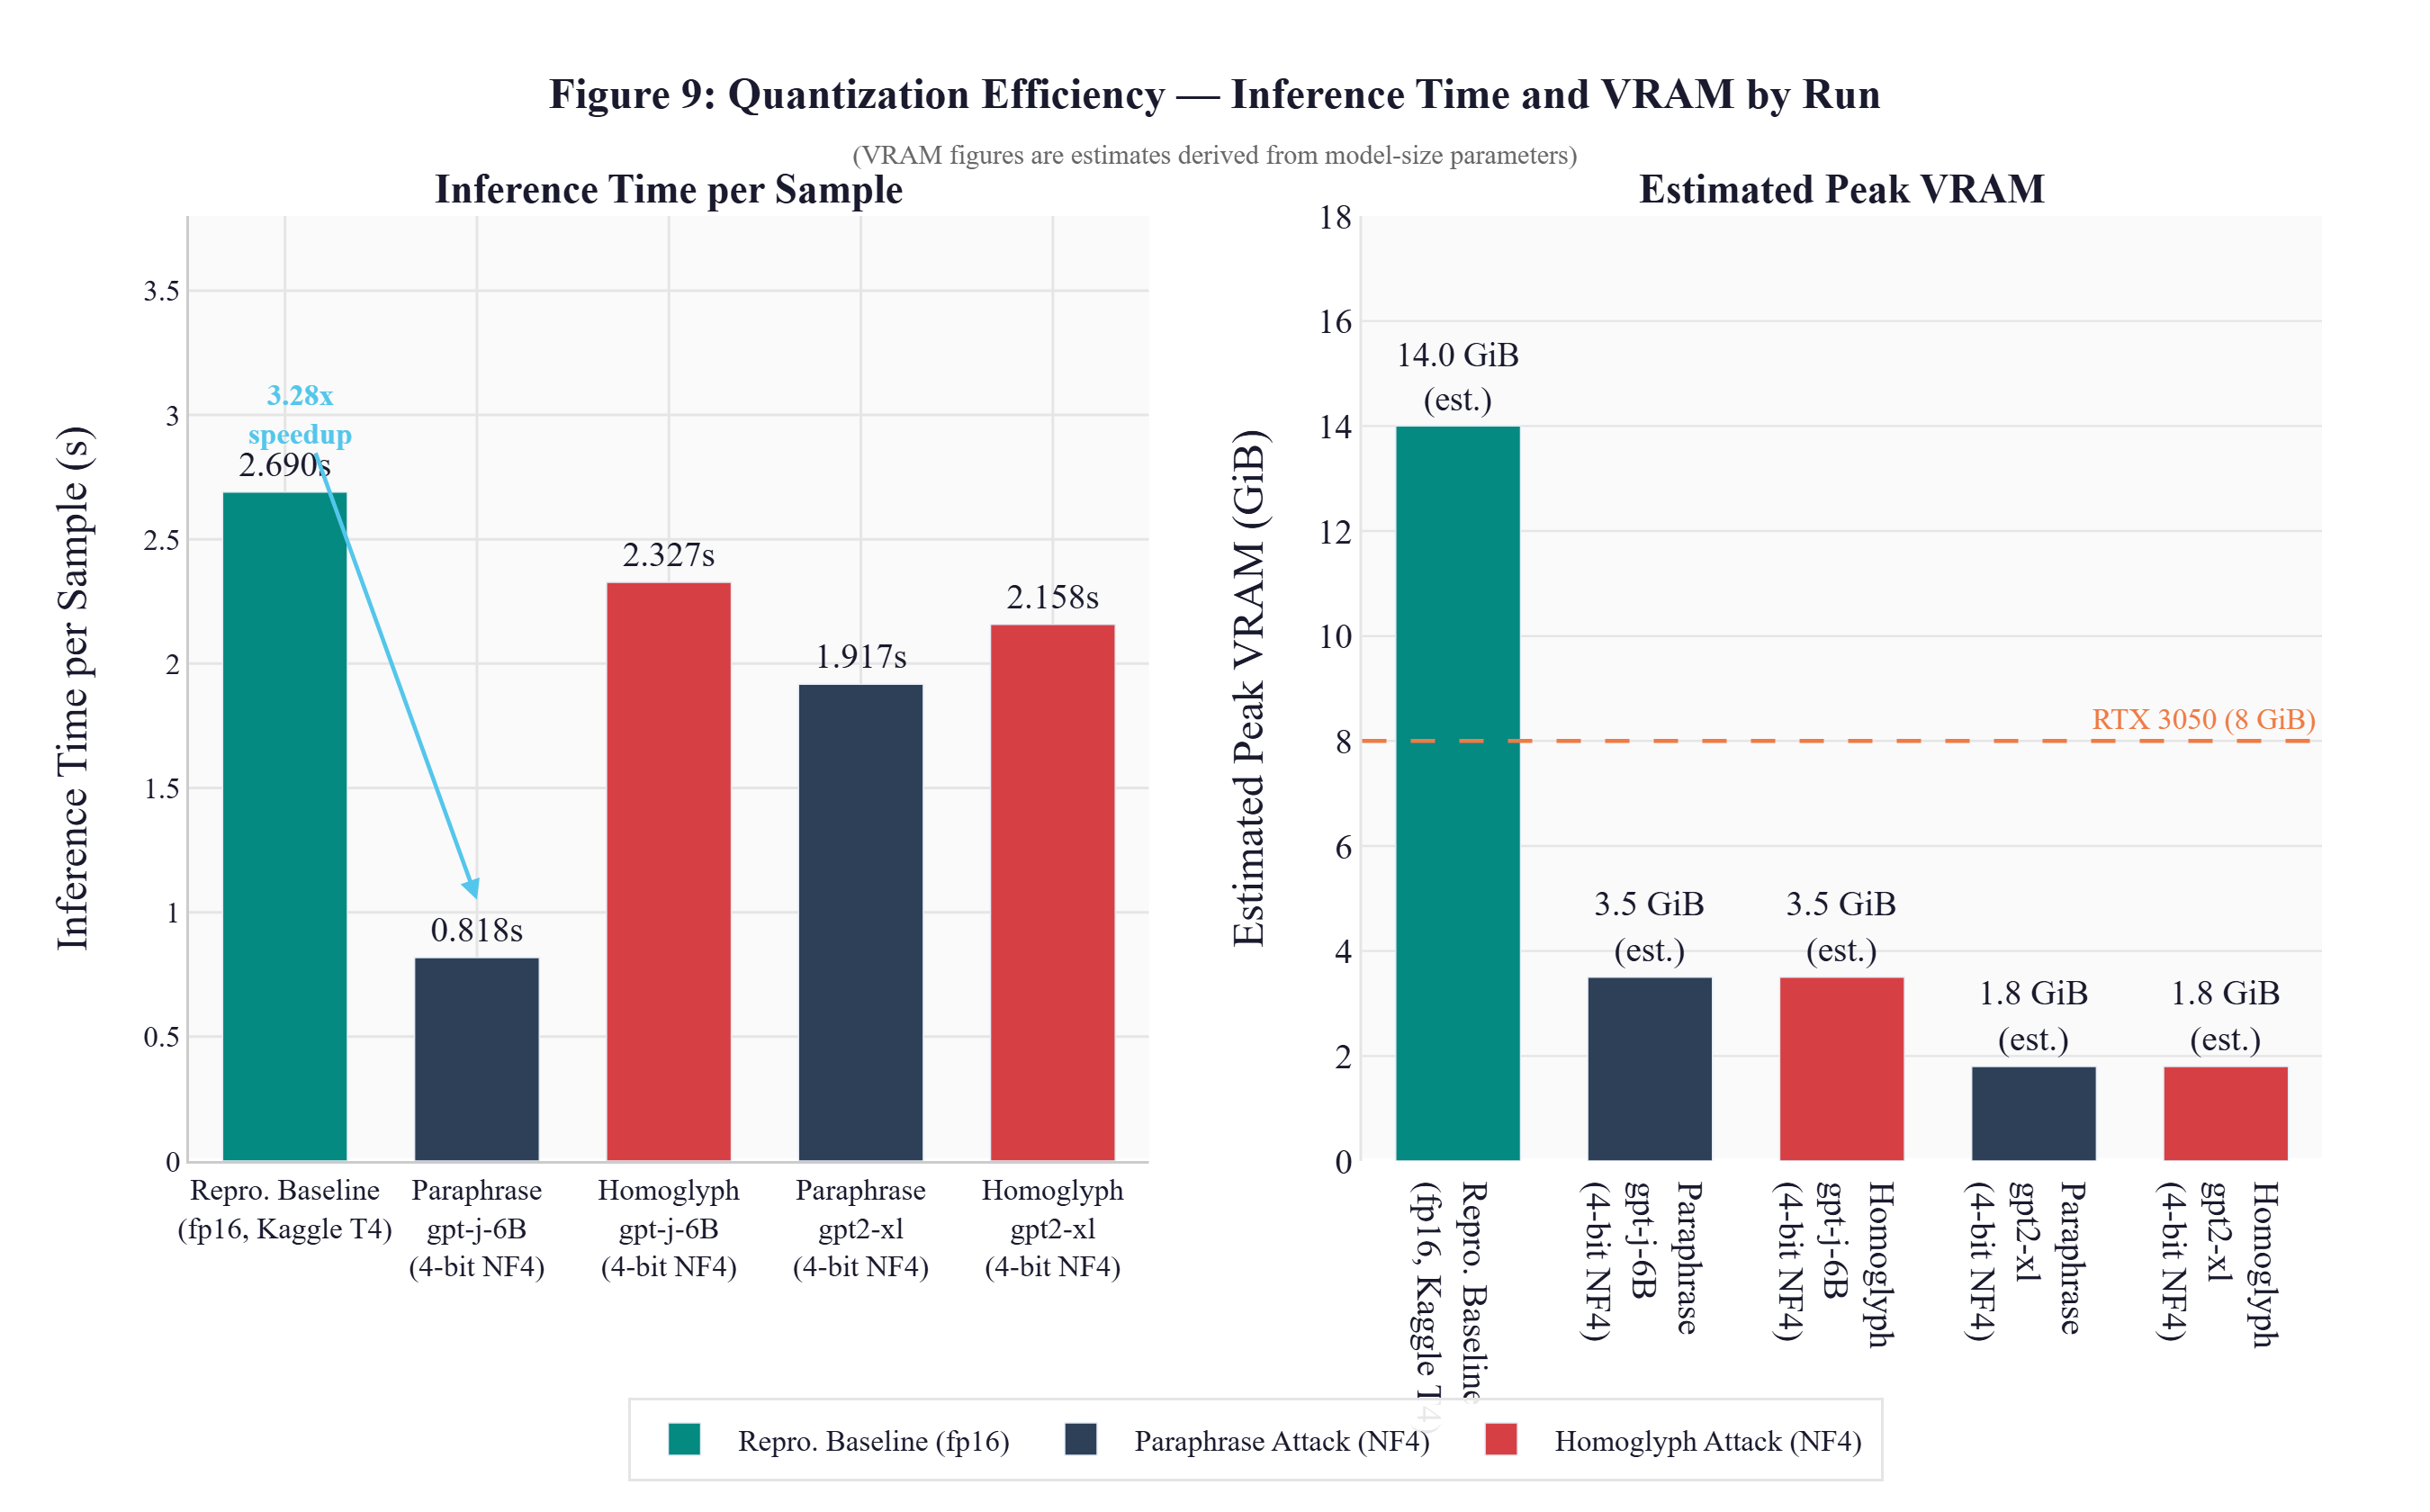
\includegraphics[width=\columnwidth]{figures/figure5_quantization_efficiency.png}
\caption{Quantisation efficiency---inference time per sample (left) and
estimated peak VRAM (right) across all experimental runs. While the 3.29$\times$ speedup
annotation on paraphrase latency (0.818~s vs. 2.690~s) reflects both model compression and 
hardware transition (T4 to RTX 4050), the VRAM chart shows the main benefit of 
4-bit NF4 quantisation: all compression configurations fall safely below the RTX~4050's 
6~GB dedicated VRAM limit (dashed orange line), preventing OOM crashes.}
\label{fig:quant}
\end{figure}

\begin{table*}[t]
\caption{Efficiency: 4-bit NF4 Quantisation vs.\ Reproduction Baseline}
\label{tab:efficiency}
\begin{center}
\small
\begin{tabular}{lcrr}
\toprule
\textbf{Condition} & \textbf{Scorer} & \textbf{Time/samp (s)} & \textbf{Est. VRAM}\\
\midrule
Repro.\ baseline (fp16, Kaggle T4) & gpt-j-6B & 2.690 (ref.)  & $\sim$14.0~GiB\\
Adversarial --- Paraphrase (NF4)   & gpt-j-6B & \textbf{0.818} & $\sim$3.5~GiB\\
Adversarial --- Homoglyph (NF4)    & gpt-j-6B & 2.327          & $\sim$3.5~GiB\\
Adversarial --- Paraphrase (NF4)   & gpt2-xl  & 1.917          & $\sim$1.8~GiB\\
Adversarial --- Homoglyph (NF4)    & gpt2-xl  & 2.158          & $\sim$1.8~GiB\\
\bottomrule
\end{tabular}
\end{center}
\end{table*}

Figure~\ref{fig:quant} and Table~\ref{tab:efficiency} show the efficiency
characteristics of the 4-bit NF4 quantised scoring setup.
Homoglyph attacks are more destructive than paraphrase
attacks for both scoring models ($p < 0.001$ in both independent
bootstrap difference tests). The \texttt{gpt2-xl} model degrades to
near-random performance under homoglyph attack (AUROC 0.5257), whereas
\texttt{gpt-j-6B} retains moderate discriminative ability (AUROC 0.6689).
The \texttt{gpt2-xl} adversarial AUROC degradation of 33.40\% suggests that attack type---rather
than quantisation level, scoring model size, or sample domain---serves as
the dominant determinant of detection difficulty under adversarial conditions.

Scoring model size provides homoglyph-specific robustness that fails to
appear under paraphrase conditions. On the paraphrase split, \texttt{gpt2-xl}
and \texttt{gpt-j-6B} perform nearly identically (AUROC 0.7893 vs.\ 0.7869,
a difference of 0.24~pp). On the homoglyph split, this gap widens to 14.3~pp.
The larger model's richer vocabulary representations retain discriminative
signal even when individual tokens suffer Unicode substitution corruption.

Although the measured 3.29$\times$ inference speedup on the paraphrase subset 
(0.818~s/sample versus the 2.690~s/sample reproduction baseline) contains a hardware 
confound due to the transition from the cloud-based Tesla~T4 to the local RTX~4050, 
the empirical validation highlights the primary systems utility of 4-bit NF4 quantisation: 
drastic VRAM reduction. Under identical hardware, 4-bit quantisation typically incurs 
a slight computational overhead due to dynamic dequantisation; however, it reduces the VRAM 
footprint by approximately 75\% for \texttt{gpt-j-6B} ($\sim$14.0~GiB $\rightarrow$ $\sim$3.5~GiB) 
and 70\% for \texttt{gpt2-xl} ($\sim$6.0~GiB $\rightarrow$ $\sim$1.8~GiB). This critical memory saving 
bridges the deployability gap, allowing models that would otherwise cause Out-Of-Memory (OOM) 
failures to run comfortably within the $\sim$6~GB dedicated VRAM ceiling of consumer laptop GPUs. 
Under homoglyph attacks, execution times increase to 2.3~s/sample, as Unicode substitutions
bypass standard tokenisation and increase per-token computation.

GPT-2 XL Perplexity's strong clean-benchmark performance does not transfer to
adversarially attacked text, regardless of quantisation efficiency.
Adversarial training or attack-aware preprocessing remains a necessary
requirement for detection pipelines deployed in real-world scenarios.

% ---------------------------------------------------------------
\section{Discussion}\label{sec:discussion}

\subsection{Held-Out-Generator Generalisation: Answering RQ1}\label{ssec:rq1}

The results provide a positive answer to RQ1 under the RAID generator split:
\emph{held-out-generator generalisation holds at the DistilBERT 66M parameter
scale}. All four ablation configurations achieve RRD values between 1.1\% and
3.1\%, remaining within the interpretive threshold of 5\% proposed in
\eqref{eq:rrd}. Held-out F1 values ranging from 0.914 to 0.927 show
competitive performance on held-out generator families not seen during training.
Addressing the second part of RQ1, DistilBERT's held-out F1 remains strong
while GPT-2 XL Perplexity degrades on RAID adversarial attack subsets (homoglyph:
AUROC 0.526--0.669; paraphrase: AUROC 0.787--0.789). Because these metrics
are not identical, the comparison should be interpreted as a directional
robustness contrast rather than a matched head-to-head score.

This outcome does not by itself resolve the cross-attack active-harm pattern
identified by Huang et al.~\cite{huang2024}, because the primary supervised
experiment here is a held-out-generator RAID evaluation rather than a clean
attack-family holdout. The result is nevertheless informative: adversarially
diverse RAID training does not collapse when the source generator family
changes. Whether the same checkpoints would preserve robustness under a
strict attack-family holdout remains an open follow-up experiment.

The generalisation performance remains notably strong even for
\texttt{baseline1}, the configuration with no layer freezing and a single-layer
head (RRD 1.11\%, held-out F1 0.9135). The base DistilBERT encoder evidently
captures representations that transfer across the seen/held-out generator
boundary independently of head complexity or freezing strategy. The ablation
study shows that architectural choices modulate the \emph{degree} of
generalisation, not its fundamental existence.

\subsection{Architectural Variable Effects: Answering RQ2}\label{ssec:rq2}

RQ2 investigates how head depth and encoder fine-tuning depth independently
affect seen-generator performance and held-out-generator robustness.

\textbf{Effect of head depth.} Comparing \texttt{ablation\_a} (single head,
freeze=4) against \texttt{ablation\_b} (deep head, freeze=4) at matched encoder
depth reveals that the deep head increases seen F1 by $+$0.72~pp
(0.9409$\rightarrow$0.9481) but raises RRD by $+$1.62~pp (1.51\%$\rightarrow$3.13\%),
exacting a cost of $-$0.83~pp in held-out F1 (0.9267$\rightarrow$0.9184). The deep
head extracts stronger in-distribution signal at a marginal cost to held-out
transfer. For deployment scenarios where seen-set precision is paramount, the
deep head is preferable; for maximum generalisation margin, the shallow head
with partial freezing performs better.

\textbf{Effect of encoder fine-tuning depth.} Comparing \texttt{ablation\_b}
(deep head, freeze=4) against \texttt{ablation\_c} (deep head, freeze=0) at
matched head architecture shows that full unfreezing raises seen ROC-AUC
by $+$0.15~pp (0.9908$\rightarrow$0.9923), raises held-out F1 by $+$0.79~pp
(0.9184$\rightarrow$0.9263), and lowers RRD by $-$0.92~pp (3.13\%$\rightarrow$2.21\%).
Full fine-tuning simultaneously improves in-distribution performance and
held-out-generator robustness. This challenges the over-fitting concern that
typically motivates partial freezing; given this dataset size and attack
distribution, the upper encoder layers actively benefit from full adaptation. The
sole trade-off is computational: unfreezing all six layers increases training
time by 1.66$\times$ relative to partial freezing (5,295~s versus 3,180~s).

\textbf{Joint recommendation.} The ablation results do not support a single
unqualified winner. \texttt{ablation\_b} is the validation-selected checkpoint
and achieves the highest seen F1, making it appropriate when checkpoint
selection and efficiency dominate. \texttt{baseline1} achieves the lowest RRD
overall, \texttt{ablation\_a} achieves the lowest RRD among the named ablations,
and \texttt{ablation\_c} achieves the strongest held-out ROC-AUC with nearly
tied held-out F1. For robustness-centric reporting, \texttt{ablation\_c} and
\texttt{ablation\_a} deserve emphasis alongside \texttt{ablation\_b}, rather
than treating \texttt{ablation\_b} as the sole proposed model.

\subsection{Systems Efficiency Insights}\label{ssec:efficiency_insights}

The four systems optimisations collectively reduce the preprocessing-to-inference
pipeline runtime from approximately 2.5~hours (cold download and sequential
processing) to under 9~seconds for preprocessing (PP), approximately
16~minutes for AMP training (AMP-T), and 84~ms/batch for inference (AMP-I).
At the 120,000-sample scale, the dominant bottleneck shifts continuously
depending on the pipeline stage. CPU-bound parallel processing governs data
preparation (PP); DataLoader overlap and memory bandwidth govern GPU feeding
(DLO); and the computation-to-memory-access ratio governs training and
inference throughput (AMP-T, AMP-I). Applying all four optimisations in
combination eliminates the dominant bottleneck at each stage to produce
additive performance gains.

The AMP-T result carries particular significance for hardware democratisation.
AMP's FP16 activations reduce VRAM consumption from the hardware ceiling
($\sim$6~GB) to 4,218.95~MB. This enables a 4$\times$ batch increase that
reduces the total gradient-step count to approximately one quarter, ultimately
yielding a 3.32$\times$ wall-clock speedup on a consumer GPU. Without AMP,
executing \texttt{batch\_size=128} remains physically infeasible on this
hardware. With AMP, a single configuration completes in under 16~minutes.

\subsection{GPT-2 XL Perplexity Adversarial Fragility}\label{ssec:perplexity_adversarial}

The RAID adversarial results clarify a structural limitation inherent to probability-based 
zero-shot detection, while also illustrating the impact of domain shift. The clean 
baseline evaluation of 0.9370 AUROC was conducted on the original \texttt{XSum/Writing/PubMed} 
corpora to establish replication fidelity. Evaluating the model on the clean-like RAID 
paraphrase subset yields 0.7893 AUROC (for \texttt{gpt2-xl}) and 0.7869 AUROC (for \texttt{gpt-j-6B}). 
This measured drop ($\sim$14.8~pp) represents a composite of both domain shift (from the 
curated Wikipedia/PubMed domains to the heterogeneous RAID Web/Recipes corpus) and paraphrase 
evasion. Under homoglyph attack on RAID, however, the degradation becomes severe: \texttt{gpt2-xl} 
drops to 0.5257 AUROC (near-random), and \texttt{gpt-j-6B} falls to 0.6689 AUROC. Crucially, 
the 4-bit NF4 quantisation yields identical AUROC performance compared to the unquantised 
reproduction baseline on paraphrase data, demonstrating that quantisation does not compound 
adversarial fragility; rather, the fragility is fundamental to the zero-shot scoring signal 
itself. Furthermore, the 4-bit NF4 quantisation enables local consumer deployment with a 
measured 3.29$\times$ per-sample speedup relative to the cloud-based FP16 reproduction baseline 
(reflecting both model compression and local hardware acceleration)~\cite{dettmers2023}.

The performance contrast between DistilBERT's held-out-generator F1
(0.913--0.927) and GPT-2 XL Perplexity's adversarial RAID AUROC (0.526--0.789)
is best read as evidence that supervised fine-tuning remains operationally
competitive under adversarial RAID conditions. A direct matched comparison
requires evaluating both systems on the same samples with the same metric.

\subsection{Limitations}\label{ssec:limits}

\subsubsection{Attack-family granularity.} The primary DistilBERT evaluation is a
held-out-generator split on RAID, not a strict attack-family holdout. The
processed held-out pool records the withheld generator identity, so it does not
support fine-grained claims about paraphrase-specific or prompt-attack-specific
F1 for the DistilBERT detector. A future version should preserve RAID's attack
labels in the held-out pool and report per-attack F1/AUROC in addition to
generator-level robustness.

\subsubsection{Hardware scope.} All DistilBERT training results originate from a
single RTX~4050~6~GB GPU. Contemporary benchmarks like GREATER~\cite{li2025} and
Binoculars~\cite{hans2024} operate on enterprise hardware requiring 28--80~GB VRAM.
Direct empirical comparison on matched hardware falls outside the resource constraints
of this study.

\subsubsection{Inference model scale.} Kaggle resource limits restricted the primary
GPT-2 XL Perplexity reproduction to \texttt{gpt-j-6B}, necessitating the exclusion of
\texttt{gpt-neox-20B}. Local adversarial runs successfully utilised both
\texttt{gpt-j-6B} and \texttt{gpt2-xl} to enable cross-scorer comparison, but this
did not replicate the full scoring model sweep present in the original publication.

\subsubsection{VRAM estimates.} Peak VRAM figures for the RAID NF4 runs serve as
estimates derived from published model-size parameters. Unreliable
\texttt{torch.cuda.reset\_peak\_memory\_stats()} behaviour between sequential
scorer loads prevented exact measurement. Actual peak VRAM may deviate from
these estimates by up to 10--15\%.

\subsubsection{Single-seed evaluation.} All DistilBERT ablation results
(Table~\ref{tab:ablation}) derive from a single training run per configuration
(seed=42). Reported values lack standard deviations or confidence intervals,
and small numerical differences between configurations (e.g., 0.9488 vs.\
0.9484 validation F1) may fall within run-to-run stochastic variation.
Multi-seed replication is needed to confirm the observed performance rankings.

\subsubsection{Absence of a clean-only training baseline.}
Every DistilBERT
configuration in this study is trained on adversarially augmented RAID data.
Without a control condition trained solely on clean (direct-prompt) AI text,
the study cannot isolate whether the observed held-out-generator robustness
is specifically attributable to adversarial augmentation or to general
properties of the DistilBERT fine-tuning procedure. A dedicated clean-only
baseline evaluated on the same held-out split would enable a direct causal
attribution of the augmentation benefit.

\subsection{Future Work}\label{ssec:future}

Several research directions follow directly from these results. Preserving RAID
attack labels in the held-out generator pool would allow per-attack F1/AUROC
reporting and a strict attack-family holdout study. Furthermore, replacing
DistilBERT with BERT-base or DeBERTa-v3-base would rigorously test whether the
observed 1.11--3.13\% RRD pattern remains specific to the distilled model scale
or successfully generalises to full-scale encoders. Finally, the severe
homoglyph vulnerability (AUROC
0.526--0.669) motivates the construction of a domain-adaptive scoring model
trained specifically on Unicode-perturbed text to harden probabilistic pipelines.

% ---------------------------------------------------------------
\section{Conclusion}\label{sec:conclusion}

We conducted a controlled empirical study evaluating held-out-generator
generalisation in supervised AI text detection at the consumer-GPU scale. A
DistilBERT binary classifier fine-tuned on adversarially augmented RAID data
achieves a Relative Robustness Degradation of 1.1--3.1\% on withheld generator
families. The model secures held-out F1 between 0.914 and 0.927, providing
positive evidence that a DistilBERT-based detector can transfer across RAID
generator families. The ablation study shows that no single
configuration dominates every criterion: \texttt{ablation\_b} is
validation-selected, \texttt{baseline1} has the lowest RRD,
\texttt{ablation\_a} has the lowest RRD among ablations, and
\texttt{ablation\_c} provides the strongest held-out ROC-AUC.

Four systems optimisations facilitate this multi-configuration training workflow on
a single 6~GB consumer GPU (RTX~4050). These include parallel preprocessing (yielding a
3.58$\times$ speedup), optimised DataLoader overlap, AMP training (yielding a
3.32$\times$ speedup and unlocking \texttt{batch\_size=128}), and AMP inference
mode (delivering a 54.25\% latency reduction). The auxiliary GPT-2 XL Perplexity
study verifies implementation fidelity (reproducing an AUROC of 0.9370 against a
0.9338 target) and shows that 4-bit NF4 quantisation does not compound
adversarial fragility. Instead, the fragility remains structurally inherent to
the probabilistic detection signal itself.

These findings are practically relevant, though the comparison is inherently
directional (the supervised and zero-shot detectors are evaluated on distinct
RAID splits using different primary metrics: held-out F1 vs.\ adversarial
AUROC). An adversarially augmented
DistilBERT model at 66M parameters, trained on standard consumer hardware in
under 16~minutes per configuration, achieves competitive held-out performance
relative to a zero-shot probabilistic detector under adversarial attack conditions.

% ---------------------------------------------------------------
\section*{Ethical Considerations}

AI text detection systems can produce consequential false positives, especially
in academic, hiring, publishing, and moderation workflows. The detector studied
here should therefore be used only as a decision-support signal, not as sole
evidence of misconduct or authorship. The adversarial results may also inform
evasion attempts; for this reason, the paper reports benchmark-level attack
categories and aggregate detector behaviour rather than operational evasion
instructions. All experiments use public benchmark datasets and derived labels;
no private user text or personally identifying data were collected.

\section*{Data and Code Availability}

The experiments use public RAID, DetectRL, and GPT-2 XL Perplexity resources.
Processed RAID splits are derived deterministically from the filtering and
training scripts using the seeds and generator-family mappings reported above.
The full project source code, configuration files, and figure-generation
scripts are publicly available at
\url{https://github.com/The-Immortal-Wanderer/Adversarially-Robust-AI-Text-Detection-via-Supervised-DistilBERT-Fine-Tuning}.

% ---------------------------------------------------------------
\section*{Acknowledgment}

The authors thank the maintainers of the GPT-2 XL Perplexity, DetectRL, and RAID
public repositories for enabling reproducible research in adversarial AI
text detection.

% ---------------------------------------------------------------
\begin{thebibliography}{99}

\bibitem{ippolito2020}
D. Ippolito, D. Duckworth, C. Callison-Burch, and D. Eck,
``Automatic detection of generated text is easiest when humans are fooled,''
in \textit{Proc. 58th Annual Meeting of the Association for Computational
Linguistics (ACL)}, 2020.



\bibitem{bao2024}
G. Bao, Y. Zhao, Z. Teng, L. Yang, and Y. Zhang,
``Fast-DetectGPT: Efficient zero-shot detection of machine-generated text
via conditional probability curvature,''
in \textit{Proc. International Conference on Learning Representations
(ICLR)}, 2024.



\bibitem{hans2024}
A. Hans, A. Schwarzschild, V. Cherepanova, H. Kazemi, A. Saha,
M. Goldblum, J. Geiping, and T. Goldstein,
``Spotting LLMs with Binoculars: Zero-shot detection of machine-generated
text,''
in \textit{Proc. 41st International Conference on Machine Learning (ICML)},
2024.



\bibitem{dugan2024}
L. Dugan, A. Hwang, F. Trhlik, J.~D. Marrow, A. Zettlemoyer,
D. Ippolito, and C. Callison-Burch,
``RAID: A shared benchmark for robust evaluation of machine-generated
text detectors,''
in \textit{Proc. 62nd Annual Meeting of the Association for Computational
Linguistics (ACL)}, 2024.



\bibitem{huang2024}
Y. Huang, D. Shi, and W. Lu,
``Towards a robust detection of language model generated text,''
in \textit{Proc. 62nd Annual Meeting of the Association for Computational
Linguistics (ACL)}, 2024.



\bibitem{sanh2019}
V. Sanh, L. Debut, J. Chaumond, and T. Wolf,
``DistilBERT, a distilled version of BERT: Smaller, faster, cheaper and
lighter,''
\textit{arXiv preprint arXiv:1910.01108}, 2019.



\bibitem{li2025}
Y. Li, Z. Zhang, C. Li, C. Shen, and X. Liu,
``Iron Sharpens Iron: Defending against attacks in machine-generated text
detection with adversarial training,''
in \textit{Proc. 63rd Annual Meeting of the Association for Computational
Linguistics (ACL)}, 2025.



\bibitem{jawahar2020}
G. Jawahar, M. Abdul-Mageed, and V.~S. Lakshmanan,
``Automatic detection of machine generated text: A critical survey,''
in \textit{Proc. 28th International Conference on Computational Linguistics
(COLING)}, 2020.



\bibitem{goodfellow2016}
I. Goodfellow, Y. Bengio, and A. Courville,
\textit{Deep Learning}.
MIT Press, 2016.



\bibitem{mitchell2023}
E. Mitchell, Y. Lee, A. Khazatsky, C.~D. Manning, and C. Finn,
``DetectGPT: Zero-shot machine-generated text detection using probability
curvature,''
in \textit{Proc. 40th International Conference on Machine Learning (ICML)},
2023.



\bibitem{hu2023}
X. Hu, P.-Y. Chen, and T.-Y. Ho,
``RADAR: Robust AI-text detection via adversarial learning,''
in \textit{Proc. 37th Annual Conference on Neural Information Processing
Systems (NeurIPS)}, 2023.



\bibitem{wu2025survey}
J. Wu, S. Yang, R. Zhan, Y. Yuan, L. S. Chao, and D. F. Wong,
``A survey on LLM-generated text detection: Necessity, methods, and future
directions,''
\textit{Computational Linguistics}, vol. 51, no. 1, pp. 275--338, 2025.



\bibitem{devlin2019}
J. Devlin, M.-W. Chang, K. Lee, and K. Toutanova,
``BERT: Pre-training of deep bidirectional transformers for language
understanding,''
in \textit{Proc. 2019 Conference of the North American Chapter of the
Association for Computational Linguistics: Human Language Technologies
(NAACL-HLT)}, 2019, pp. 4171--4186.



\bibitem{he2021}
P. He, X. Liu, J. Gao, and W. Chen,
``DeBERTa: Decoding-enhanced BERT with disentangled attention,''
in \textit{Proc. International Conference on Learning Representations
(ICLR)}, 2021.



\bibitem{kirchenbauer2023}
J. Kirchenbauer, J. Geiping, Y. Wen, J. Katz, I. Miers, and T. Goldstein,
``A watermark for large language models,''
in \textit{Proc. 40th International Conference on Machine Learning (ICML)},
2023.



\bibitem{tufts2025}
B. Tufts, X. Zhao, and L. Li,
``A practical examination of AI-generated text detectors for large language
models,''
in \textit{Findings of the Association for Computational Linguistics:
NAACL 2025}, 2025, pp. 4839--4856.



\bibitem{pedrotti2025}
A. Pedrotti, M. Papucci, C. Ciaccio, A. Miaschi, G. Puccetti,
F. Dell'Orletta, and A. Esuli,
``Stress-testing machine generated text detection: Shifting language models
writing style to fool detectors,''
in \textit{Findings of the Association for Computational Linguistics:
ACL 2025}, 2025, pp. 3010--3031.



\bibitem{zha2025padben}
Y. Zha, R. Min, and S. Sushmita,
``PADBen: A comprehensive benchmark for evaluating AI text detectors against
paraphrase attacks,''
\textit{arXiv preprint arXiv:2511.00416}, 2025.



\bibitem{baidya2026}
M. S. Baidya, S. S. Baidya, and C. Chawla,
``Detecting the machine: A comprehensive benchmark of AI-generated text
detectors across architectures, domains, and adversarial conditions,''
\textit{arXiv preprint arXiv:2603.17522}, 2026.



\bibitem{wu2024detectrl}
J. Wu, R. Zhang, and W. Ma,
``DetectRL: Benchmarking LLM-generated text detection in real-world
scenarios,''
in \textit{Proc. 38th Annual Conference on Neural Information Processing
Systems (NeurIPS)}, 2024.



\bibitem{isenko2022}
A. Isenko, R. Mayer, J. Jedele, and H.-A. Jacobsen,
``Where is my training bottleneck? Hidden trade-offs in deep learning
preprocessing pipelines,''
in \textit{Proc. 2022 International Conference on Management of Data
(SIGMOD)}, 2022.



\bibitem{dettmers2023}
T. Dettmers, A. Pagnoni, A. Holtzman, and L. Zettlemoyer,
``QLoRA: Efficient finetuning of quantized LLMs,''
in \textit{Proc. 37th Annual Conference on Neural Information Processing
Systems (NeurIPS)}, 2023.



\end{thebibliography}

\end{document}
